%% ============================================================
%% Journal of Communication and Information Systems (JCIS)
%% Submission version -- IEEE Transactions two-column template.
%%
%% JCIS requires the IEEE Transactions template in two-column
%% format, English text, a DOI for every reference, and the ORCID
%% of every author at submission time.
%%
%% Compile with:  pdflatex -> bibtex -> pdflatex -> pdflatex
%% Requires:      IEEEtran.cls and IEEEtran.bst (ship with the
%%                official IEEE template) and referencias.bib.
%% ============================================================
\documentclass[journal]{IEEEtran}

% ---- Math ----
\usepackage{amsmath,amssymb,amsfonts}
\usepackage{amsthm}
\newtheorem{lemma}{Lemma}
\interdisplaylinepenalty=2500   % restore IEEEtran page breaks after amsmath

% ---- Algorithms ----
\usepackage{algorithm}
\usepackage{algorithmic}

% ---- Tables ----
\usepackage{array}
\usepackage{booktabs}

% ---- Figures / subfigures ----
\usepackage{graphicx}
\usepackage[caption=false,font=normalsize,labelfont=sf,textfont=sf]{subfig}

% ---- Misc ----
\usepackage{textcomp}
\usepackage{stfloats}
\usepackage{url}
\usepackage{cite}            % proper IEEE-style numeric citation sorting
\hyphenation{Lya-pu-nov non-li-near}

\begin{document}

% ============================================================
% TITLE AND AUTHORS
% ============================================================
\title{Analysis of the Chaotic Regime in the Filtered H\'enon Map}
\author{Kau\^e~de~Souza~Silva,
        Roger~Freitas~Pereira,
        Marcos~Felipe~Correa~Soares,
        Guilherme~Rodrigues~dos~Santos,
        and~Vin\'icius~da~Silva~Borges%
\thanks{K. de S. Silva is an undergraduate student in Computer Engineering
at the Faculdade Engenheiro Salvador Arena (FESA), Centro Educacional da
Funda\c{c}\~ao Salvador Arena, Estrada dos Alvarengas, 4001, S\~ao Bernardo
do Campo, SP, Brazil. ORCID: 0009-0009-1283-0996 (e-mail:
kaue.moelas.com@gmail.com).}%
\thanks{R. F. Pereira is an undergraduate student in Computer Engineering
at FESA, S\~ao Bernardo do Campo, SP, Brazil. ORCID: 0009-0000-5624-7422
(e-mail: roger\_freitas@live.com).}%
\thanks{M. F. C. Soares is an undergraduate student in Computer Engineering
at FESA, S\~ao Bernardo do Campo, SP, Brazil. ORCID: 0009-0009-9968-2227
(e-mail: marcosfelipe.soares2014@gmail.com).}%
\thanks{G. R. dos Santos is an undergraduate student in Computer Engineering
at FESA, S\~ao Bernardo do Campo, SP, Brazil. ORCID: 0009-0004-0281-8663
(e-mail: guilhermerodriguess130@gmail.com).}%
\thanks{V. da S. Borges is with the Computer Engineering Department, FESA,
S\~ao Bernardo do Campo, SP, Brazil. He is the academic advisor of this
work. ORCID: 0000-0001-5546-6842 (e-mail: viniciussbrg@gmail.com).}%
}

% Running headers (edit volume/number once JCIS assigns them)
\markboth{Journal of Communication and Information Systems,~Vol.~XX, No.~X, Month~Year}%
{Silva \MakeLowercase{\textit{et al.}}: Analysis of the Chaotic Regime in the Filtered H\'enon Map}

\maketitle

% ============================================================
% ABSTRACT
% ============================================================
\begin{abstract}
The insertion of finite impulse response (FIR) filters in the feedback
loop of chaotic generators is a known strategy for bandwidth
limitation in chaos-based communication systems (CBCS). However, the
interplay between the nonlinearity of the generating map and the
linearity of the filter may disrupt the chaotic regime, compromising the
application. This work systematically characterizes, by means of
numerical simulations, the conditions under which chaos is preserved in
the two-dimensional H\'enon map with internal FIR filters, considering
four filter types (lowpass, highpass, bandpass, and bandstop) and seven
design windows, with a dedicated sweep over the Kaiser window. The
largest Lyapunov exponent is estimated by the tangent-map method with
Modified Gram--Schmidt orthonormalization over an ensemble of initial conditions
centered at the equilibrium point of the expanded system, and the
protocol is validated against the standard map. Bootstrap confidence
intervals on the exponent quantify the statistical confidence of the
chaotic-coverage estimates. The implementation is delivered as an open-source Python
package with JIT-compiled cores via Numba and dedicated data-versioning
and automated-testing infrastructure. Results show that FIR filters do
not eliminate the chaotic regime but rather reorganize it into
geometrically intricate regions of the parameter space---interleaving chaotic,
periodic, and divergent zones---whose shape
depends systematically on the filter type and the design window
employed.
\end{abstract}

\begin{IEEEkeywords}
Chaos-based communication systems, H\'enon map, FIR filters, Lyapunov
exponent.
\end{IEEEkeywords}

% ============================================================
\section{Introduction}\label{sec:intro}
% ============================================================
\IEEEPARstart{I}{nformation} security in communication systems has
traditionally been provided by encryption techniques at the upper layers
of the reference model. In parallel, physical-layer security seeks to
exploit the characteristics of the medium and of the transmitted signal
itself in order to hinder interception by unauthorized receivers, without
relying exclusively on upper-layer encryption~\cite{Mukherjee2014}.
In this context, chaos-based communication systems (CBCS) are among the
approaches under study: by employing chaotic signals as information
carriers, they exploit properties such as the wideband spectrum and the
noise-like appearance of these signals~\cite{Baptista2021}.

A deterministic discrete-time chaotic signal has three characteristics
that distinguish it from classical periodic or stochastic
signals~\cite{Alligood1996}: it is amplitude-bounded, aperiodic, and
exhibits sensitive dependence on initial conditions (SDIC), that is, two
orbits initially arbitrarily close diverge exponentially in phase space
after a finite time~\cite{Henon1976}. These properties motivated, starting
from the seminal work of Pecora and Carroll~\cite{Pecora1990}, the use of
chaotic signals in telecommunications and signal processing. Pecora and
Carroll~\cite{Pecora1990} showed that two identical chaotic-signal
generators can be synchronized, despite SDIC, when the receiver is driven
by state variables of the transmitter. Such synchronization-based schemes
fall within the broader class of \emph{coherent} CBCS, as opposed to
\emph{non-coherent} architectures, which recover the transmitted
information from statistical or structural properties of the received
signal without reconstructing a synchronized replica at the
receiver~\cite{Kaddoum2016}. Since then, multiple CBCS
applications have been proposed: modulation schemes~\cite{Baptista2021},
image coding and encryption~\cite{Sabatini2020}, systems based on
three-dimensional attractors~\cite{Souza2019}, and, more recently, schemes
with chaotic phase-locked loops~\cite{Silva2025sbrt}.

A fundamental issue when applying chaotic signals to communication systems
is the spectral width. Because transmission channels are always
band-limited, it is necessary to know and \emph{limit} the bandwidth of the
transmitted chaotic signals---not to control it arbitrarily, but to confine
it within the channel passband~\cite{Eisencraft2011}. To this end,
Eisencraft \textit{et al.}~\cite{Eisencraft2009} proposed the use of
discrete-time linear filters embedded in the chaotic-signal generator, and
Fontes \textit{et al.}~\cite{Fontes2016} consolidated the approach by
showing that inserting the filter does not prevent chaotic synchronization.
The behavior of the system under additional practical limitations, such as
the digitalization of the numerical representation, was later investigated
by Borges \textit{et al.}~\cite{Borges2021sbrt}.

A central question in this approach is whether the signals generated by the
system with an inserted filter remain chaotic, given that the filter
modifies the dynamics of the original generating map. This question has been
investigated by Borges and Eisencraft~\cite{Borges2022sbrt,BorgesCSF2022},
who showed numerically, for low-order FIR filters, that the filter
coefficients affect the behavior of the generated signals, with phenomena
such as bifurcation cascades, coexistence of attractors, crises, and
periodicity islands of the \textit{shrimp} type~\cite{Gallas1993}. Borges
\textit{et al.}~\cite{BorgesCNSNS2024} extended the analysis to FIR filters
with a larger number of coefficients and different zero placements, and
Borges \textit{et al.}~\cite{Borges2024sbrt} to second-order all-pole
filters. These works establish that the chaotic regime is not guaranteed to
survive filtering and must be verified case by case---the starting point of
the present study.

Whereas~\cite{BorgesCNSNS2024} characterized the filtered H\'enon map across
different zero-placement geometries of the FIR filter with a fixed design
window, the present investigation
treats \emph{frequency selectivity} and \emph{window design} as the primary
axes. In addition to lowpass FIR filters, highpass, bandpass, and bandstop
filters are considered, each designed through seven distinct windows, with a
dedicated parametric sweep of the Kaiser shape parameter~\cite{Kaiser1980}.
Through high-resolution dynamic classification maps in the filter
order--cutoff frequency plane, we show that the preservation of chaos is
governed, in a structured and only partly monotonic way, by the filter type
and the design window: stopband attenuation correlates positively with
chaotic coverage for lowpass, highpass, and bandpass filters, but the
relation \emph{reverses} for bandstop, where the low-attenuation rectangular
window dominates. Aggregating the 124 sweeps further exposes a
configuration-robust region of the order--cutoff plane in which chaos
persists across windows and filter types. Relative to the previously published numerical
characterizations of the filtered H\'enon map by Borges \textit{et
al.}~\cite{Borges2022sbrt,BorgesCSF2022,BorgesCNSNS2024}, which vary the
zero-placement geometry of the FIR filter with a fixed design window, the
present work adds
two directions proper to computer engineering: (i)~a statistical
characterization of the chaotic coverage, with bootstrap confidence
intervals on the Lyapunov exponent; and (ii)~a description of the
computational architecture of the implemented pipeline---a Python package
with cores compiled by Numba~\cite{Numba}, parallelization over the
parameter grid, checkpoint versioning, and automated testing---as a
condition for scientific reproducibility.

The objective of this work is to characterize systematically the conditions
under which the chaotic regime is preserved in the H\'enon map with an
internal FIR filter, sweeping the order--cutoff frequency plane for four
filter types and seven design windows. To this end, the largest Lyapunov
exponent is estimated by the tangent-map method with Modified Gram--Schmidt
orthonormalization and validated against the standard H\'enon map; the
resulting orbits are classified into high-resolution dynamic maps for the
four filter types and seven windows; the effect of the Kaiser-window shape
parameter $\beta_K$ on the chaotic coverage is assessed; the chaotic-coverage
estimates are accompanied by bootstrap confidence intervals on the exponent;
and the whole pipeline is documented and released as a reproducible
artifact~\cite{chaoticPFC2026}. This work covers the filter order, the cutoff
frequency, the filter type, and the design window; other dimensions of the
parameter space are left as future work enabled by the released infrastructure.

The remainder of this paper is organized as follows. Section~\ref{sec:theory}
presents the theoretical background (H\'enon map, expanded system with FIR
filter, the frequency-domain rationale for feedback filtering, design
windows, and Lyapunov exponent); Section~\ref{sec:method}
describes the experimental methodology, including the computational
architecture of the pipeline; Section~\ref{sec:results} presents and
discusses the results; and Section~\ref{sec:conclusion} summarizes the
conclusions and proposes future work.

% ============================================================
\section{Theoretical Background}\label{sec:theory}
% ============================================================
This section presents the theoretical tools used throughout the work, in
the order in which they will be mobilized in the following sections.
Subsection~\ref{sub:henon} defines the two-dimensional H\'enon map, its
expanded version under internal FIR filtering, and the corresponding
Jacobian matrix. Subsection~\ref{sub:freq} motivates, from a master--slave
synchronization standpoint, why the feedback filter must be specified and
evaluated in the frequency domain. Subsection~\ref{sub:windows} describes
the seven FIR design windows considered. Subsection~\ref{sub:lyap}
formalizes the Lyapunov exponent, the tangent-map recursion with
Gram--Schmidt orthogonalization, and the adopted dynamic-classification
criterion.

% ---- 2.1 ----
\subsection{H\'enon Map and Expanded System With FIR Filter}\label{sub:henon}
The two-dimensional H\'enon map~\cite{Henon1976} is the discrete dynamical
system adopted in this work as the chaotic generator. In its standard
two-dimensional form, it is written as
\begin{equation}
  \begin{cases}
    x_1(n+1) = \alpha - x_1^2(n) + \beta\, x_2(n), \\
    x_2(n+1) = x_1(n),
  \end{cases}
  \label{eq:henon}
\end{equation}
where $\alpha$ and $\beta$ are real parameters. For $\alpha = 1.4$ and
$\beta = 0.3$, the map produces a strange attractor whose largest Lyapunov
exponent is $\lambda_1\approx 0.42$ and whose fractal dimension is
$\approx 1.26$~\cite{Alligood1996,BorgesCSF2022,Henon1976}. The Lyapunov
exponent measures the average exponential rate at which two nearby orbits
separate and thus quantifies the SDIC; it is formally defined in
Subsection~\ref{sub:lyap}, and for the present purposes it is enough to note
that a positive $\lambda_1$ is the signature of chaos. From the
dissipative relation $\det\mathbf{J} = -\beta$, with $|\beta|<1$, follows
the identity $\lambda_1 + \lambda_2 = \ln|\beta|$, valid for the
two-dimensional system and used here as a consistency test for the
implemented Lyapunov estimator (Subsection~\ref{sub:validation}).

As proposed by Eisencraft \textit{et al.}~\cite{Eisencraft2009} and
Fontes \textit{et al.}~\cite{Fontes2016}, the bandwidth of the generated
signals can be limited by filtering $x_1(n)$ through an FIR filter
with $N_s$ coefficients $c_j$, $0\le j\le N_s-1$, according to
\eqref{eq:filtro}:
\begin{equation}
  x_3(n) = \sum_{j=0}^{N_s-1} c_j\, x_1(n-j),
  \label{eq:filtro}
\end{equation}
and feeding $x_3(n)$ back into the system in place of $x_1(n)$ in the
nonlinear term. The filter order is $N_z = N_s - 1$, equal to the
number of zeros of the transfer function~\cite{Oppenheim2009}. Because the
filter in \eqref{eq:filtro} depends on the $N_s$ most recent values of
$x_1$, the instantaneous pair $(x_1,x_2)$ is no longer a complete state of
the system: the past samples $x_1(n-1),\ldots,x_1(n-N_s+1)$ must also be
stored for the next iteration to be determined. To recover a first-order
(memoryless) description, these delayed samples are kept as
\emph{auxiliary state variables} $x_4,\ldots,x_{N_s}$, each of which simply
holds a one-step delay of the preceding variable. With this augmentation,
for $N_s>3$, the system is written in the expanded state-space form of
Borges \textit{et al.}~\cite{Borges2022sbrt,BorgesCNSNS2024}, reproduced in
\eqref{eq:expandido}:
\begin{equation}
  \begin{cases}
    x_1(n+1) = \alpha - x_3^2(n) + \beta\, x_2(n), \\
    x_2(n+1) = x_1(n), \\
    x_3(n+1) = c_0\bigl(\alpha - x_3^2(n) + \beta\, x_2(n)\bigr) + c_1\, x_1(n) \\
    \qquad\qquad + c_2\, x_2(n) + c_3\, x_4(n) + \cdots + c_{N_s-1}\, x_{N_s}(n), \\
    x_4(n+1) = x_2(n), \\
    x_j(n+1) = x_{j-1}(n),\quad j = 5,\ldots,N_s,
  \end{cases}
  \label{eq:expandido}
\end{equation}
where the last two lines are precisely the delay chain that stores the
filter memory.
The dimension of the expanded system is $K = N_s$ (equal to the number of
coefficients); for $N_s=1$ (identity filter $c_0=1$) the original
two-dimensional map~\eqref{eq:henon} is recovered. A \emph{fixed point}
(also called an \emph{equilibrium point}) of a discrete map $\mathbf{F}$ is a
state $\mathbf{x}^\star$ that is left unchanged by one iteration,
$\mathbf{x}^\star = \mathbf{F}(\mathbf{x}^\star)$; an orbit started exactly at
$\mathbf{x}^\star$ stays there for all $n$~\cite{Alligood1996}. For the
two-dimensional map~\eqref{eq:henon}, solving
$\mathbf{x}^\star = \mathbf{F}(\mathbf{x}^\star)$ gives two fixed points,
of which the positive one is the relevant reference state. The same
condition applied to the expanded system~\eqref{eq:expandido} defines its
positive fixed point $\mathbf{p}^+$, which depends on the
total gain $G = \sum_j c_j$ of the filter---equal to the filter gain
at $\omega = 0$, i.e., its DC gain~\cite{Oppenheim2009}---and can be obtained
analytically following~\cite{BorgesCNSNS2024}; this property is used in the
initialization of the ensemble of initial conditions
(Subsection~\ref{sub:ensemble}).

The Jacobian matrix of system~\eqref{eq:expandido}, evaluated at instant
$n$, is given by~\cite{Borges2022sbrt,BorgesCNSNS2024}
\begin{equation}
  \mathbf{J}(n) = \begin{pmatrix}
    0 & \beta & -2x_3(n) & 0 & \cdots & 0 \\
    1 & 0 & 0 & 0 & \cdots & 0 \\
    c_1 & \beta c_0 & -2c_0 x_3(n) & c_3 & \cdots & c_{N_s-1} \\
    0 & 1 & 0 & 0 & \cdots & 0 \\
    \vdots & & & \ddots & & \vdots \\
    0 & \cdots & 0 & 0 & 1 & 0
  \end{pmatrix},
  \label{eq:jacobiana}
\end{equation}
of dimension $K\times K$ with $K=N_s$. Only the third row of
$\mathbf{J}(n)$ depends explicitly on the filter coefficients $\{c_j\}$,
showing that the entire interaction between the linear dynamics introduced
by the filter and the quadratic nonlinearity of the map is concentrated in
that state equation. This structure partially explains why the total gain
$G = \sum_j c_j$ is a relevant scalar parameter of the dynamic
behavior of the expanded system~\cite{BorgesCNSNS2024}.

% ---- 2.2 ----
\subsection{Frequency-Domain Rationale for Filtering the Feedback Loop}\label{sub:freq}
The reason the filter in~\eqref{eq:filtro} must be designed and evaluated in
the frequency domain, rather than treated as an arbitrary linear
combination of past samples, becomes clear once~\eqref{eq:henon} is
embedded in a coherent chaos-based communication architecture of the
master--slave type~\cite{Pecora1990}. Let $\mathbf{x}(n)$ and
$\mathbf{y}(n)$ denote the state vectors of an autonomous transmitter
(master) and a driven receiver (slave), respectively, and let
$\mathbf{e}(n)\triangleq\mathbf{y}(n)-\mathbf{x}(n)$ be the synchronization
error. When the nonlinearity acts on a single scalar carrier extracted
from the state---as in~\eqref{eq:henon}, where that role is played by
$x_1(n)$---the error dynamics reduce to the linear recursion
\begin{equation}
  \mathbf{e}(n+1) = \mathbf{A}\,\mathbf{e}(n),
  \label{eq:syncerror}
\end{equation}
where $\mathbf{A}$ is the synchronization matrix; synchronization is
attained whenever every eigenvalue $\lambda_k(\mathbf{A})$, $1\le k\le K$,
lies strictly inside the unit circle, $|\lambda_k(\mathbf{A})|<1$
~\cite{BorgesTese2026}. Under an ideal, distortion-free channel this
condition is sufficient for the receiver to track the transmitter
asymptotically and for the transmitted message to be recovered without
degradation, apart from an initial transient.

Real transmission channels, however, are never distortion-free: physical
limitations of the medium impose a finite passband, so the channel acts as
a filter that reshapes the spectrum of the transmitted
signal~\cite{Eisencraft2011}. Because chaotic carriers spread their energy
continuously over a wide band rather than concentrating it on a few
spectral lines~\cite{Baptista2021}, even a modest truncation of that
spectrum is enough to unsettle the coherent receiver: the driven
(slave) system no longer evolves under the same effective nonlinearity as
the master, the synchronization error ceases to vanish, and the recovered
message estimate no longer tracks the original waveform, in either the
time or the frequency domain~\cite{BorgesTese2026}. Confining the
transmitted spectrum to the channel passband \emph{before} transmission is
therefore not an optional refinement but a precondition for coherent
detection over bandlimited channels~\cite{Eisencraft2009,Fontes2016}.

The FIR branch of~\eqref{eq:filtro} implements exactly this pre-shaping
inside the feedback loop, and its two equivalent descriptions make the
frequency-domain interpretation explicit. In the time domain,
$x_3(n)$ is a finite convolution of $x_1(n)$ with the coefficients
$\{c_j\}$; taking the $z$-transform of~\eqref{eq:filtro} under zero
initial conditions yields the transfer function $H(z) = X_3(z)/X_1(z) =
\sum_{j=0}^{N_s-1} c_j z^{-j}$, whose evaluation on the unit circle,
$H(e^{j\omega})$, is the frequency response that fixes the passband,
transition width, and stopband attenuation actually delivered by a given
choice of $\{c_j\}$~\cite{Oppenheim2009}. It is this frequency response,
not the raw coefficient values, that must be matched to the channel
bandwidth---which is precisely why the filter order $N_z$ and the cutoff
frequency $\omega_c$, rather than the individual $c_j$, are adopted as the
sweep variables of the present study (Subsection~\ref{sub:grid}), and why
the design method reviewed in Subsection~\ref{sub:windows} operates
directly on that frequency response.

Embedding the filter in the feedback path, rather than only at the channel
interface, has a further consequence for the synchronization matrix
$\mathbf{A}$ itself, formalized next.

\begin{lemma}[Synchronizability under FIR feedback filtering, adapted
from~\cite{BorgesTese2026}]\label{lem:sync}
Let the master--slave pair satisfy the synchronization condition
$|\lambda_k(\mathbf{A})|<1$, $1\le k\le K$. Inserting an FIR filter of
order $N_z$ in the feedback path, as in~\eqref{eq:expandido}, enlarges the
synchronization matrix to dimension $(K+N_z)\times(K+N_z)$ by adding only
null eigenvalues. Hence the original condition remains sufficient,
independently of the coefficients $\{c_j\}$.
\end{lemma}

Synchronizability of the master--slave
pair is therefore preserved for \emph{any} choice of coefficients
$\{c_j\}$, provided the unfiltered pair already synchronizes---a
guarantee that holds regardless of how aggressively the filter shapes the
spectrum. This result, however, concerns only the linear stability of
$\mathbf{e}(n)$; it says nothing about whether the master's own
trajectory $\mathbf{x}(n)$ remains chaotic once the same coefficients
$\{c_j\}$ are fed back nonlinearly through~\eqref{eq:expandido} and enter
the Jacobian in~\eqref{eq:jacobiana}. Synchronization and chaoticity are
thus two logically independent requirements: the former is guaranteed by
construction, while the latter---as already anticipated in
Section~\ref{sec:intro} and demonstrated numerically for low-order filters
by Borges \textit{et al.}~\cite{Borges2022sbrt,BorgesCSF2022,BorgesCNSNS2024}---is
not. Consequently, a frequency-domain specification of $H(z)$ that merely
fits the channel passband cannot, by itself, certify that the filtered
generator remains a valid chaotic source; it must be complemented by the
explicit dynamical verification developed in the remainder of this paper.
This distinction motivates treating the window used to synthesize $H(z)$
as a first-class design variable, reviewed next.

% ---- 2.3 ----
\subsection{FIR Design Windows}\label{sub:windows}
The FIR filters are designed by the method of windowing the ideal impulse
response~\cite{Oppenheim2009,Harris1978}, a technique that establishes a
direct trade-off between stopband attenuation and transition-band width.
Seven windows are investigated, as summarized in Table~\ref{tab:windows}.
The attenuation values listed there are the peak side-lobe levels of each
window's discrete-time Fourier transform, measured relative to the main-lobe
peak; in the windowing method this side-lobe level fixes the minimum stopband
attenuation that the resulting FIR filter can attain~\cite{Harris1978,Oppenheim2009}.
The values grow from $21$~dB for the rectangular window---whose abrupt
truncation of the impulse response produces strong side lobes---to $92$~dB for
the four-term Blackman--Harris window, whose cosine-sum coefficients are
chosen precisely to cancel side lobes~\cite{Harris1978}; this gain in
attenuation is paid for with a wider main lobe and therefore a wider
transition band.

The Hamming window is adopted as a historical reference because it was used
in the original works of Fontes \textit{et al.}~\cite{Fontes2016} and Borges
and Eisencraft~\cite{Borges2022sbrt} on the filtered H\'enon map. The
Kaiser window~\cite{Kaiser1980}, parameterized by $\beta_K\ge 0$, allows the
trade-off between attenuation and transition width to be varied continuously
without changing the filter order---for $\beta_K = 0$ it degenerates into the
rectangular window, and typical values $\beta_K\in[2,14]$ yield windows whose
attenuations correspond to those of the Bartlett, Hamming, Blackman, or
Blackman--Harris windows~\cite{Oppenheim2009}.

\begin{table}[!t]
\caption{FIR Windows Evaluated and Their Typical Stopband Attenuations\label{tab:windows}}
\centering
\begin{tabular}{lcc}
\toprule
\textbf{Window} & \textbf{Atten. (dB)} & \textbf{Characteristic} \\
\midrule
Rectangular (boxcar)          & 21       & Minimum reference \\
Bartlett                      & 25       & Triangular \\
Hamming                       & 41       & Standard reference \\
Hann                          & 44       & Raised cosine \\
Blackman                      & 74       & High attenuation \\
Blackman--Harris              & 92       & Maximum attenuation \\
Kaiser ($\beta_K$ variable)   & variable & Parametric \\
\bottomrule
\end{tabular}

\vspace{2pt}
{\footnotesize Source: adapted from~\cite{Harris1978} and~\cite{Oppenheim2009}.}
\end{table}

The seven selected windows cover a broad spectrum of trade-offs between
transition-band width and stopband attenuation: the rectangular window as
the worst case, the Bartlett and Hann windows as classical intermediates,
the Hamming window as the reference adopted in the previous filtered-H\'enon
literature~\cite{Fontes2016,Borges2022sbrt}, and the Blackman and
Blackman--Harris windows as representatives of high-attenuation
windows---under the hypothesis that greater spectral attenuation favors the
preservation of the chaotic regime by reducing side-lobe leakage into the
rejected band. The Kaiser window, with $\beta_K$ swept over 25 values,
provides a continuous path connecting these regimes. The design of the
coefficients $\{c_j\}$ is carried out by the \texttt{firwin} routine of the
SciPy library~\cite{Virtanen2020}.

% ---- 2.4 ----
\subsection{Lyapunov Exponent and Dynamic Classification}\label{sub:lyap}
By \emph{sensitivity} here we mean the sensitive dependence on initial
conditions (SDIC) introduced in Section~\ref{sec:intro}: how fast two orbits
that start arbitrarily close to each other drift apart as the system evolves.
This rate is made quantitative by the Lyapunov exponent, defined as the
natural logarithm of the average factor by which the separation between two
nearby orbits is multiplied at each iteration. An exponent equal to $\ln 2$
along a given coordinate means, for example, that the distance between the
orbits doubles at every iteration in that direction, on
average~\cite{Alligood1996,Wolf1985}; a negative exponent means the orbits
converge in that direction. For a discrete system of dimension $K$ there are
$K$ such exponents, one per coordinate of the tangent space, and the SDIC of
the generated signals is characterized by the largest of them, $\lambda_1$.

The tangent-map method is adopted~\cite{Alligood1996,Wolf1985}. Consider a
unit-radius hypersphere centered at the initial condition $\mathbf{x}(0)$,
represented by a matrix $\mathbf{U}$ whose columns are orthonormal vectors.
At each iteration, this hypersphere is transformed into an ellipsoid by the
product of the Jacobian matrix $\mathbf{J}(n)$ of the expanded system, given
by \eqref{eq:jacobiana}. To avoid numerical divergence or collapse of the
axes along the iterations, Gram--Schmidt orthogonalization is applied at each
step to the set
$\{\mathbf{J}(n)\mathbf{w}_1(n),\ldots,\mathbf{J}(n)\mathbf{w}_K(n)\}$. The
recursion of the orthonormal basis is therefore
\begin{equation}
  \begin{split}
    \mathbf{y}_k(n+1) ={}& \mathbf{J}(n)\,\mathbf{w}_k(n) \\
    &- \sum_{j=1}^{k-1}\bigl\langle\mathbf{J}(n)\mathbf{w}_k(n),\,
    \mathbf{w}_j(n+1)\bigr\rangle\,\mathbf{w}_j(n+1),
  \end{split}
  \label{eq:tangentrec}
\end{equation}
\begin{equation}
  \mathbf{w}_k(n+1) = \frac{\mathbf{y}_k(n+1)}{\|\mathbf{y}_k(n+1)\|},
  \qquad 1\le k\le K,
  \label{eq:tangentnorm}
\end{equation}
where the summation in~\eqref{eq:tangentrec} implements the Gram--Schmidt
orthogonalization against the vectors already orthogonalized in the same
iteration, and the normalization in~\eqref{eq:tangentnorm} preserves the
orthonormal character of the basis along the iterations; $K$ is the
dimension of the expanded system~\cite{Borges2022sbrt}. The Lyapunov
exponent in the $k$-th direction is then
\begin{equation}
  \lambda_k = \lim_{n\to\infty}
  \frac{\ln\|\mathbf{y}_k(1)\| + \cdots + \ln\|\mathbf{y}_k(n)\|}{n}.
  \label{eq:lyap}
\end{equation}

The \emph{orbit} of an initial condition $\mathbf{x}(0)$ is the sequence of
states $\{\mathbf{x}(n)\}_{n\ge 0}$ produced by iterating the map; it is
\emph{bounded} when there exists a finite $M$ such that
$\|\mathbf{x}(n)\|\le M$ for all $n$, and \emph{divergent} otherwise. The
dynamic classification adopted for each point of the parameter grid is
\begin{equation}
  \begin{cases}
    \lambda_1 > 0    & \rightarrow \text{chaotic}, \\
    \lambda_1 \le 0  & \rightarrow \text{periodic or stationary},
  \end{cases}
  \label{eq:criterio}
\end{equation}
\textit{conditioned} on the boundedness of the orbit. The case
$\lambda_1\le 0$ groups two asymptotically non-chaotic behaviors:
convergence to an equilibrium point (fixed point) of the
system---defined in Subsection~\ref{sub:henon} as the state
$\mathbf{x}^\star$ satisfying $\mathbf{x}^\star=\mathbf{F}(\mathbf{x}^\star)$---and
convergence to a periodic orbit~\cite{Alligood1996}. Both are grouped into
the ``periodic or stationary'' class, because the criterion of this work
distinguishes only the presence ($\lambda_1>0$) or absence
($\lambda_1\le 0$) of chaos, and not the specific period of the limit orbit.
First, however, it is necessary to separate the orbits that remain bounded
from those that escape: the regime is classified as \textit{divergent} when
the state vector satisfies $\|\mathbf{x}(n)\| > X_{\max}$ for some $n$ along
the iteration, with $X_{\max} = 10^{6}$ adopted in this work. In that case,
$\lambda_1$ is discarded, since the boundedness hypothesis underlying
\eqref{eq:lyap} no longer holds.

The criteria and equations presented in this section underpin the
experimental methodology described next, in which \eqref{eq:lyap} is
evaluated by numerical simulation over a dense grid of the filter parameter
space.

% ============================================================
\section{Methodology}\label{sec:method}
% ============================================================
This section describes the experimental methodology, organized so that each
design decision is introduced before it is used. Subsection~\ref{sub:arch}
discusses the computational architecture that makes the parameter sweep
tractable; Subsection~\ref{sub:types} lists the filter types and windows
evaluated; Subsection~\ref{sub:grid} specifies the sweep grid;
Subsection~\ref{sub:estimator} details the implementation of the Lyapunov
estimator; Subsection~\ref{sub:ensemble} describes the ensemble of initial
conditions and the global parameters; Subsection~\ref{sub:metrics} defines the
chaotic-coverage metrics; Subsection~\ref{sub:stats} introduces the statistical
quantification; and Subsection~\ref{sub:repro} summarizes the reproducibility
infrastructure.

The research adopts a quantitative-experimental approach. All the tooling
was implemented in the Python package \texttt{chaotic\_pfc}, released as
open source under the BSD-3-Clause license~\cite{chaoticPFC2026}, with sweep
cores compiled via Numba~\cite{Numba} for parallel execution over the
parameter grid. Each submodule referenced in this section corresponds to a
module of the package, and the technical documentation in Sphinx is
published via Read the Docs~\cite{chaoticPFC2026}.

% ---- 3.1 ----
\subsection{Computational Architecture of the Pipeline}\label{sub:arch}
Systems with SDIC impose characteristic computational constraints that
deserve treatment within the scope of computer engineering. Reliable
estimation of $\lambda_1$ requires long simulation horizons (hundreds to
thousands of iterations per orbit) and an ensemble of initial conditions to
mitigate sensitivity to transients~\cite{Wolf1985}. Parametric sweeps in the
$(N_z,\omega_c/\pi)$ plane, even at moderate resolution, generate thousands
of independent points, each with its own ensemble: for a
$40\times 100\times 25$ grid (filter order, cutoff frequency, initial
conditions), a single sweep demands $10^5$ evaluations of the Lyapunov
estimator.

Three architectural decisions were adopted in the pipeline. First,
Just-In-Time (JIT) compilation of the numerical cores via Numba~\cite{Numba},
which translates annotated Python functions into machine code through LLVM,
with a reduction of one to two orders of magnitude in execution time relative
to the pure-Python fallback, as measured by the package
benchmarks~\cite{chaoticPFC2026}.
Second, explicit parallelization over the $(N_z,\omega_c/\pi)$ grid by means
of \texttt{prange} loops, exploiting all the cores available on the host
machine. Third, versioning of the sweep checkpoints as compressed NumPy files
(\texttt{.npz}), allowing figures and tables to be recomputed without redoing
the sweeps---a scientific-reproducibility requirement recommended for
published computational artifacts.

The complexity of the Lyapunov estimator per grid point is dominated by the
QR orthogonalization, $\mathcal{O}(K^3)$ per step, and by the
Jacobian--basis product, $\mathcal{O}(K^2)$ per step, where
$K = N_s = N_z+1$ is the dimension of the expanded system. For
$N_{\text{map}}$ accumulation iterations and $N_{\text{IC}}$ initial
conditions, the total cost per grid point is
$\mathcal{O}(N_{\text{IC}}\cdot N_{\text{map}}\cdot K^3)$. For high orders
($N_z=40$, $K=41$), $N_{\text{map}}=3{,}000$ and $N_{\text{IC}}=25$, the cost
approaches $5\times 10^9$ floating-point operations per grid point, making
JIT compilation a practical requirement rather than a luxury.

% ---- 3.2 ----
\subsection{Filter Types and Windows Evaluated}\label{sub:types}
Four FIR filter types are investigated: lowpass, highpass, bandpass, and
bandstop, all designed by the windowing method with the seven windows listed
in Table~\ref{tab:windows}. For the band filters (bandpass and bandstop), the
total width is fixed at $\Delta\omega = 0.05\,\pi$, distributed symmetrically
around the center frequency $\omega_c$. This value is a deliberate compromise.
On the normalized axis $\omega/\pi\in(0,1)$ it corresponds to a band of $5\%$
of the available range, which spans about five steps of the cutoff grid (100
values over the open interval, Subsection~\ref{sub:grid}); the band is
therefore narrow enough to keep the filter clearly frequency-selective---a
genuine bandpass or bandstop rather than a near-allpass---yet wide enough to
be resolved by the sweep and to admit a non-degenerate pass/stop band at every
$\omega_c$. Fixing $\Delta\omega$ also isolates the effect of the single
geometric parameter under study, the center frequency $\omega_c$; the band
width is left as an independent variable for future work
(Section~\ref{sec:conclusion}).

The design of the coefficients is carried out by
\texttt{scipy.signal.firwin}, wrapped by the FIR-design routines of the
package. For
highpass and bandstop filters, the parity restriction of the windowing method
requires $N_z$ to be even~\cite{Oppenheim2009}, otherwise the filter ceases to
have a null response at the desired frequency; this restriction is honored by
the package when building the grid.

% ---- 3.3 ----
\subsection{Parameter Sweep Grid}\label{sub:grid}
For lowpass and bandpass filters, $N_z\in\{1,2,\ldots,40\}$ is swept with 100
values of normalized cutoff frequency $\omega_c/\pi$ linearly spaced in the
open interval $(0,1)$, totaling $4{,}000$ points per window--filter
configuration. For highpass and bandstop filters, the parity restriction of
the windowing method requires $N_z$ to be even~\cite{Oppenheim2009}, reducing
the set to $N_z\in\{2,4,\ldots,40\}$, with $2{,}000$ points per configuration.
For the Kaiser window, an additional dedicated sweep covers
$\beta_K\in[2.0,14.0]$ with step $0.5$ (25 values) for the four filter types,
totaling 100 additional Kaiser configurations. Adding the combinations with
fixed windows ($4\times 6 = 24$), the experiment covers 124 sweeps.

% ---- 3.4 ----
\subsection{Lyapunov Estimator: Implementation}\label{sub:estimator}
Algorithm~\ref{alg:lyap} summarizes the implementation of the Lyapunov
estimator adopted in the \texttt{lyapunov.py} module, based on the
formulation of Wolf \textit{et al.}~\cite{Wolf1985} adapted to
system~\eqref{eq:expandido}. The QR orthogonalization uses the Modified
Gram--Schmidt algorithm, numerically more stable than the classical one when
the tangent vectors become nearly parallel after many iterations.

\begin{algorithm}[!t]
\caption{Lyapunov spectrum estimation by tangent map with Modified Gram--Schmidt.}\label{alg:lyap}
\begin{algorithmic}[1]
\STATE \textbf{Input:} initial condition $\mathbf{x}_0$; burn-in iterations $N_{\text{burn}}$; accumulation iterations $N_{\text{map}}$; divergence threshold $X_{\max}$.
\STATE $\mathbf{W}\leftarrow\mathbf{I}_{K}$;\; $\boldsymbol{\lambda}\leftarrow\mathbf{0}$;\; $\mathbf{x}\leftarrow\mathbf{x}_0$.
\FOR{$i=1$ \TO $N_{\text{burn}}$}
  \STATE $\mathbf{x}\leftarrow\mathbf{F}(\mathbf{x})$ \quad(discard transient).
\ENDFOR
\FOR{$i=1$ \TO $N_{\text{map}}$}
  \STATE $\mathbf{x}\leftarrow\mathbf{F}(\mathbf{x})$ \quad(orbit evolution).
  \IF{$\|\mathbf{x}\|>X_{\max}$}
    \STATE \textbf{return} \textsc{NaN} \quad(divergent orbit).
  \ENDIF
  \STATE $\mathbf{Z}\leftarrow\mathbf{J}(\mathbf{x})\cdot\mathbf{W}$ \quad(tangent-map evolution).
  \STATE $(\mathbf{Q},\mathbf{R})\leftarrow\mathrm{MGS}(\mathbf{Z})$; extract $n_k = |\mathbf{R}_{kk}|$.
  \STATE $\lambda_k \mathrel{+}{=} \ln\max(n_k,10^{-300})$, $1\le k\le K$.
  \STATE $\mathbf{W}\leftarrow\mathbf{Q}$.
  \STATE \textit{(early stop)} every 100 iterations, if the variation of $\lambda_1$ stayed below $\varepsilon = 10^{-3}$ for two consecutive checkpoints and $i \ge 500$, terminate.
\ENDFOR
\STATE \textbf{return} $\boldsymbol{\lambda}/i$.
\end{algorithmic}
\end{algorithm}

The early-stop step substantially reduces the computational cost without
compromising accuracy: the criterion of \textit{two} consecutive checkpoints
mitigates premature stops in windows of chaotic intermittency (in which
$\lambda_1$ oscillates for hundreds of iterations before stabilizing).

% ---- 3.5 ----
\subsection{Ensemble of Initial Conditions and Global Parameters}\label{sub:ensemble}
For each grid point $(N_z,\omega_c)$, 25 initial conditions are sampled
uniformly in a cube of edge $\epsilon = 0.1$ around the positive equilibrium
point $\mathbf{p}^+$ of the expanded system, computed analytically from the
total gain $G=\sum_j c_j$~\cite{BorgesCNSNS2024}. The estimator of
Subsection~\ref{sub:estimator} is run with $N_{\text{burn}} = 500$ discard
iterations before accumulation over $N_{\text{map}} = 3{,}000$ iterations. The
value reported for the point is the mean of $\lambda_1$ over the ensemble,
classified according to criterion~\eqref{eq:criterio}.

The choice of $N_{\text{burn}} = 500$ stems from the estimate of the
characteristic relaxation time to the attractor in the standard H\'enon map
($\sim 1/\lambda_1\approx 2.4$ iterations), with an ample margin to accommodate
longer transients in configurations close to bifurcation boundaries. The
accumulation horizon $N_{\text{map}} = 3{,}000$ corresponds to approximately
$10^3/\lambda_1$ in this standard case, sufficient to reduce the standard
deviation of the estimate below $10^{-2}$---a verification reported in
Subsection~\ref{sub:validation}.

In all experiments: $\alpha = 1.4$ and $\beta = 0.3$ (standard parameters of
the H\'enon map); $\beta_K = 5.0$ in the general Kaiser-window sweep; and the
pseudo-random generator seed fixed at $42$, for reproducibility.

% ---- 3.6 ----
\subsection{Chaotic Coverage Metrics}\label{sub:metrics}
Each grid point is labelled, by the criterion of Subsection~\ref{sub:lyap}, as
chaotic, periodic/stationary, or divergent. Let $N_{\text{grid}}$ be the total
number of grid points, $N_b$ the number of points whose orbit is bounded
(chaotic or periodic, i.e., non-divergent), and $N_c$ the number of chaotic
points. Two complementary chaotic-coverage metrics are then reported. The
\emph{conditional} fraction $\rho_c^{\text{fin}} = N_c/N_b$ is the share of
chaotic points among the bounded ones; it measures the propensity to chaos
once numerical stability is ensured, deliberately excluding the divergent
region so that it is not artificially deflated. The \emph{absolute} fraction
$\rho_c^{\text{abs}} = N_c/N_{\text{grid}}$ is taken over the whole grid and
measures the usable fraction of the design space. The two metrics answer
different design questions: $\rho_c^{\text{fin}}$ is relevant when the designer
can adjust $N_z$ and $\omega_c$ to reach a specific non-divergent operating
point, whereas $\rho_c^{\text{abs}}$ is relevant when a broad operating range
with few divergent configurations is sought. The difference in grid size
($4{,}000$ points for lowpass and bandpass against $2{,}000$ for highpass and
bandstop) follows from the parity restriction on $N_z$ inherent to the
windowing method~\cite{Oppenheim2009}; the comparisons between filter types use
fractions precisely to neutralize this difference in sample size.

% ---- 3.7 ----
\subsection{Statistical Treatment of the Sweep Results}\label{sub:stats}
The statistical characterization operates at two distinct levels, which are
kept separate to avoid ambiguity. At the \emph{point} level, the value of
$\lambda_1$ reported for each grid point $(N_z,\omega_c)$ is the mean over the
ensemble of $N_{\text{IC}}=25$ initial conditions (Subsection~\ref{sub:ensemble}),
and the per-point ensemble dispersion is retained as metadata. At the
\emph{regional} level, the chaotic region of a given window--filter
configuration is summarized by the mean, standard deviation, and a $95\%$
confidence interval of $\lambda_1$ computed \emph{over the set of chaotic grid
points} of that configuration (sample size equal to $N_c$). It is this regional
mean---not the per-point ensemble mean---whose confidence interval is reported
in Tables~\ref{tab:best} and~\ref{tab:ranking}; consequently, the standard
deviation $\sigma_{\lambda_1}$ measures the spatial homogeneity of the chaotic
region rather than estimation noise at a single point. The interval is obtained
by nonparametric bootstrap~\cite{EfronTibshirani1993} with $1{,}000$ resamples
and a fixed seed ($42$), so that it quantifies the sampling variability of the
regional mean over the chaotic set. The corresponding routines are in the
module \texttt{chaotic\_pfc/analysis/stats.py} of the released
package~\cite{chaoticPFC2026}.

% ---- 3.8 ----
\subsection{Reproducibility Infrastructure}\label{sub:repro}
Each complete sweep generates a \texttt{.npz} file containing the tensor
$\lambda_1(N_z,\omega_c)$ over the ensemble, the classification vector, the
coefficients of the filters used, and the execution metadata (seed, code hash,
timestamp). The files are versioned in \texttt{data/sweeps/} via Git LFS,
allowing figures and tables to be recomputed without recomputing the sweeps.
Automated tests (in \texttt{tests/}) verify, at each repository commit: the
identity $\lambda_1+\lambda_2 = \ln|\beta|$ in the canonical map, the accuracy
of the $\lambda_1$ estimate against the reference value
of~\cite{Alligood1996}, and the consistency of the designed filters
(coefficient sum, zero placement). Continuous integration runs the tests at
each code change.

All the infrastructure described here is available as open source under the
BSD-3-Clause license~\cite{chaoticPFC2026}, with a Git version tag and a
\texttt{CITATION.cff} file following the FORCE11 recommendations for the
citation of scientific software. The technical documentation in Sphinx is
published on Read the Docs and contains the description of each module, with
usage examples and the API reference.

% ============================================================
\section{Results and Discussion}\label{sec:results}
% ============================================================
This section presents and discusses the results of the parametric sweeps
conducted according to the methodology of Section~\ref{sec:method}.
Subsection~\ref{sub:validation} validates the Lyapunov estimator against the
standard, unfiltered H\'enon map; Subsection~\ref{sub:classification} consolidates the
configurations of greatest chaotic coverage by filter type;
Subsections~\ref{sub:maps} and~\ref{sub:density} detail the classification
maps and the aggregate density; Subsection~\ref{sub:beta} addresses the effect
of the Kaiser-window parameter $\beta_K$; Subsection~\ref{sub:ranking} reports
the statistical significance of the estimates and the ranking of the
combinations; and Subsection~\ref{sub:cost} discusses the computational cost
and reproducibility. Results original to this work are reported in direct
prose; observations that reproduce previous findings of Borges and Eisencraft
\cite{Borges2022sbrt,BorgesCSF2022,BorgesCNSNS2024} are marked as ``confirms''
or ``is consistent with''; statements from the general literature are marked
with a reference to their source.

% ---- 4.1 ----
\subsection{Estimator Validation}\label{sub:validation}
The estimation protocol was validated on the \emph{standard} H\'enon
map---the original, unfiltered two-dimensional map of \eqref{eq:henon} with
the classical parameters $\alpha=1.4$, $\beta=0.3$ (recovered by setting
$N_s = 1$, $c_0 = 1$), often referred to as the \emph{canonical} case---for
which the literature establishes
$\lambda_1\approx 0.42$~\cite{Alligood1996,BorgesCSF2022,Wolf1985}.
The run with the parameters described in Section~\ref{sec:method} (ensemble of
25 initial conditions, $N_{\text{burn}} = 500$, $N_{\text{map}} = 3{,}000$,
seed 42, early stop disabled) reproduced $\bar\lambda_1 = 0.4182$, with a
relative error below $10^{-2}$. This level of accuracy is sufficient to
distinguish the dynamic regimes defined in~\eqref{eq:criterio}. In addition,
the identity $\lambda_1 + \lambda_2 = \ln|\beta|$---a direct consequence of the
dissipation of the map---was satisfied to machine precision in all unfiltered
configurations tested, confirming the algorithmic correctness of the estimator
independently of the published reference value. In the subsequent sweeps, the
early stop (Subsection~\ref{sub:estimator}) is enabled to reduce the
computational cost.

% ---- 4.2 ----
\subsection{Dynamic Classification of the Parameter Space}\label{sub:classification}
Table~\ref{tab:best} consolidates, for each filter type, the configuration
that maximizes the absolute number of chaotic points $N_c$ in the parametric
sweep, considering both the fixed-coefficient windows and the Kaiser window
with the $\beta_K$ that maximizes $N_c$. As a comparative reference, the
second configuration in decreasing order of $N_c$ is also reported (a fixed
window for lowpass, highpass, and bandpass; Kaiser for bandstop, in which the
first position is occupied by the rectangular window).

\begin{table*}[!t]
\caption{Configuration of Largest $N_c$ per Filter Type, With Mean, Standard Deviation, and Confidence Interval of $\lambda_1$\label{tab:best}}
\centering
\begin{tabular}{llrrrrrc}
\toprule
\textbf{Filter} & \textbf{Window} & $N_c$ &
$\rho_c^{\text{fin}}$ & $\rho_c^{\text{abs}}$ &
$\bar\lambda_1$ & $\sigma_{\lambda_1}$ & 95\% CI of $\bar\lambda_1$ \\
\midrule
Lowpass   & Kaiser ($\beta_K{=}13.5$) & 979 & 77.6\% & 24.5\% & 0.0239 & 0.0231 & $[0.0223,\,0.0254]$ \\
          & Blackman--Harris          & 961 & 74.8\% & 24.0\% & 0.0211 & 0.0232 & $[0.0197,\,0.0227]$ \\
\midrule
Highpass  & Kaiser ($\beta_K{=}11.5$) & 149 &  8.1\% &  7.5\% & 0.0178 & 0.0263 & $[0.0138,\,0.0219]$ \\
          & Blackman--Harris          & 144 &  7.9\% &  7.2\% & 0.0190 & 0.0269 & $[0.0151,\,0.0237]$ \\
\midrule
Bandpass  & Kaiser ($\beta_K{=}13.5$) & 434 & 13.0\% & 10.8\% & 0.0286 & 0.0297 & $[0.0258,\,0.0315]$ \\
          & Blackman--Harris          & 418 & 12.3\% & 10.4\% & 0.0261 & 0.0301 & $[0.0235,\,0.0293]$ \\
\midrule
Bandstop  & Rectangular               & 118 & 65.2\% &  5.9\% & 0.0709 & 0.0491 & $[0.0627,\,0.0800]$ \\
          & Kaiser ($\beta_K{=}4.0$)  &  58 & 39.2\% &  2.9\% & 0.0726 & 0.0336 & $[0.0626,\,0.0798]$ \\
\bottomrule
\end{tabular}

\vspace{2pt}
{\footnotesize 95\% confidence intervals obtained by
bootstrap~\cite{EfronTibshirani1993}. Full per-configuration tables are regenerated from the versioned
checkpoints by the released package~\cite{chaoticPFC2026}.}
\end{table*}

The Kaiser window leads in three of the four filter types, both in
$\rho_c^{\text{fin}}$ and in $\rho_c^{\text{abs}}$. However, this comparison
must be interpreted with caution, since each fixed window corresponds to a
single coefficient configuration per grid point, whereas the Kaiser window was
evaluated at 25 values of $\beta_K$, giving it a higher sampling density.
Disregarding Kaiser, the Blackman--Harris window is the dominant reference for
lowpass, highpass, and bandpass---a result consistent with its higher spectral
attenuation (92\,dB) and suggesting a positive association between window
attenuation and preservation of the chaotic regime in these three filter
types.

The bandstop filter constitutes a particular case: the rectangular window
reaches $\rho_c^{\text{fin}} = 65.2\%$, the highest conditional fraction among
all filter types. This is consistent with the DC-gain argument developed in
Subsection~\ref{sub:maps}: the bandstop filter rejects only a narrow band
($\Delta\omega = 0.05\,\pi$) away from $\omega=0$, so its DC gain
$G=\sum_j c_j$ remains close to unity, keeping the positive fixed point
$\mathbf{p}^+$ well defined; bounded orbits then inherit a structured dynamics
and are predominantly chaotic. In absolute terms, however, its coverage is
modest ($\rho_c^{\text{abs}} = 5.9\%$) because a large share of the grid is
divergent at higher orders, as detailed in Subsection~\ref{sub:maps}.

The lowpass filter with the Kaiser window ($\beta_K=13.5$) reaches the highest
absolute coverage among the 124 window--filter combinations swept in this work,
with $\rho_c^{\text{abs}} = 24.5\%$ against the $5.9\%$ of the bandstop---a
ratio of approximately $4.2\times$ in absolute coverage, or $8.3\times$ in the
number of chaotic points ($979$ against $118$).

% ---- 4.3 ----
\subsection{Classification Maps}\label{sub:maps}
Figures~\ref{fig:lowpass}--\ref{fig:bandstop} present the dynamic
classification maps in the $(N_z,\omega_c/\pi)$ plane for the configuration of
largest $N_c$ of each filter type, colored according to
criterion~\eqref{eq:criterio}: red for chaotic, blue for periodic, and gray
for divergent.

The dynamic reading of these maps reinforces, now across four filter types and
seven windows, two observations previously reported by Borges \textit{et
al.}~\cite{BorgesCNSNS2024,BorgesCSF2022}. First, the total filter gain
$G = \sum_j c_j$ scales the positive fixed point $\mathbf{p}^+$
of the expanded system; values of $G$ close to zero shift $\mathbf{p}^+$ toward
regions in which the term $\alpha - x_3^2$ tends to diverge, which in our maps
appears as the gray (divergent) regions that dominate high orders and certain
$\omega_c$---corroborating the analytical dependence of $\mathbf{p}^+$ on $G$
established in~\cite{BorgesCNSNS2024}. Second,
the thin boundaries between chaotic and periodic regions are period-doubling
bifurcation cascades, and the periodic islands inside the chaotic regions are
\textit{shrimps}~\cite{Gallas1993}---periodic structures characteristic of
two-dimensional quadratic maps, whose occurrence in the filtered H\'enon map
was first documented by Borges and Eisencraft~\cite{BorgesCSF2022}; our sweeps
confirm that they persist across all four filter types studied here.

\begin{figure}[!t]
\centering
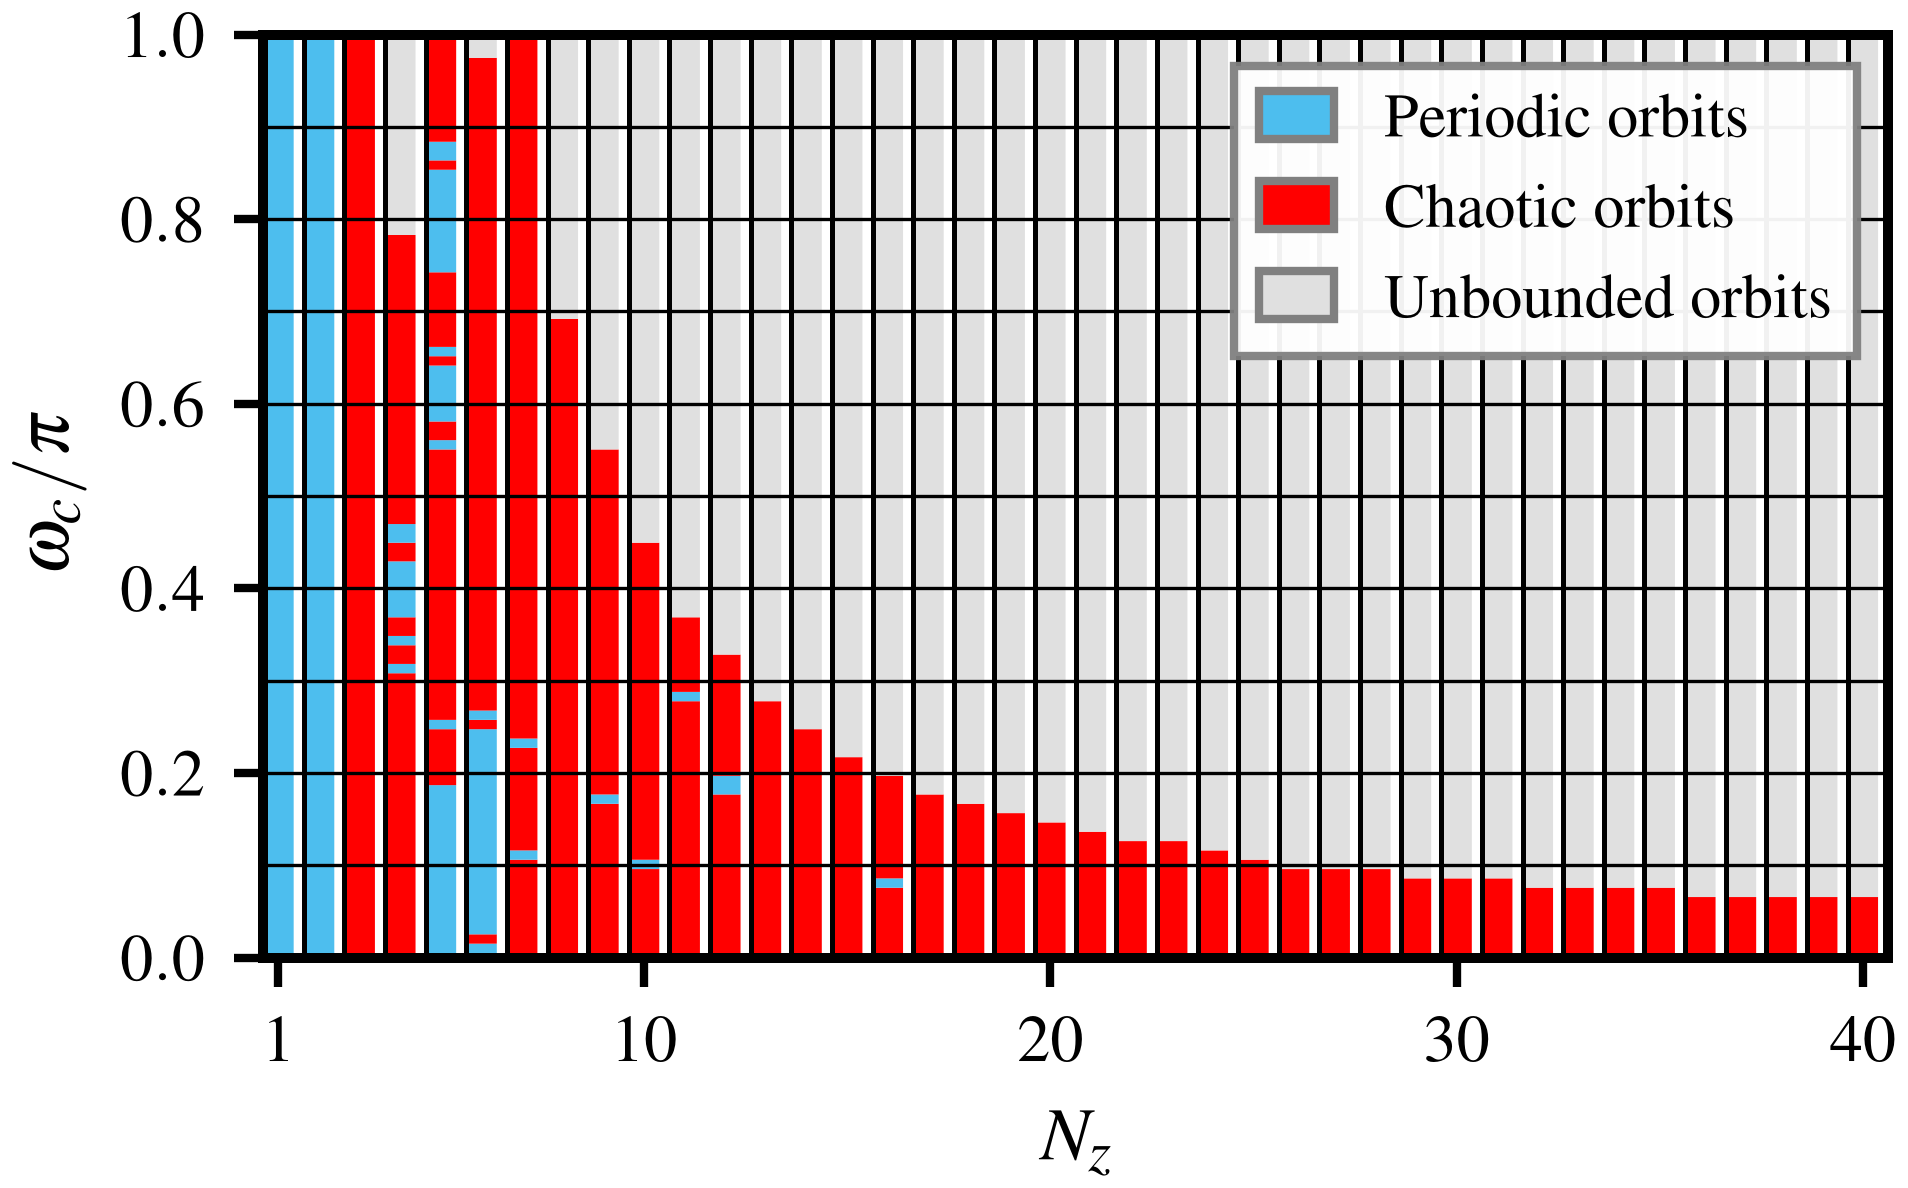
\includegraphics[width=\columnwidth]{Figures/kaiser_b13p5_lowpass_classification_interleaved.png}
\caption{Lowpass, Kaiser ($\beta_K=13.5$). A wide chaotic region for
$\omega_c/\pi\gtrsim 0.2$, with periodicity islands (\textit{shrimps}) at low
orders. The divergent region grows with $N_z$.}
\label{fig:lowpass}
\end{figure}

\begin{figure}[!t]
\centering
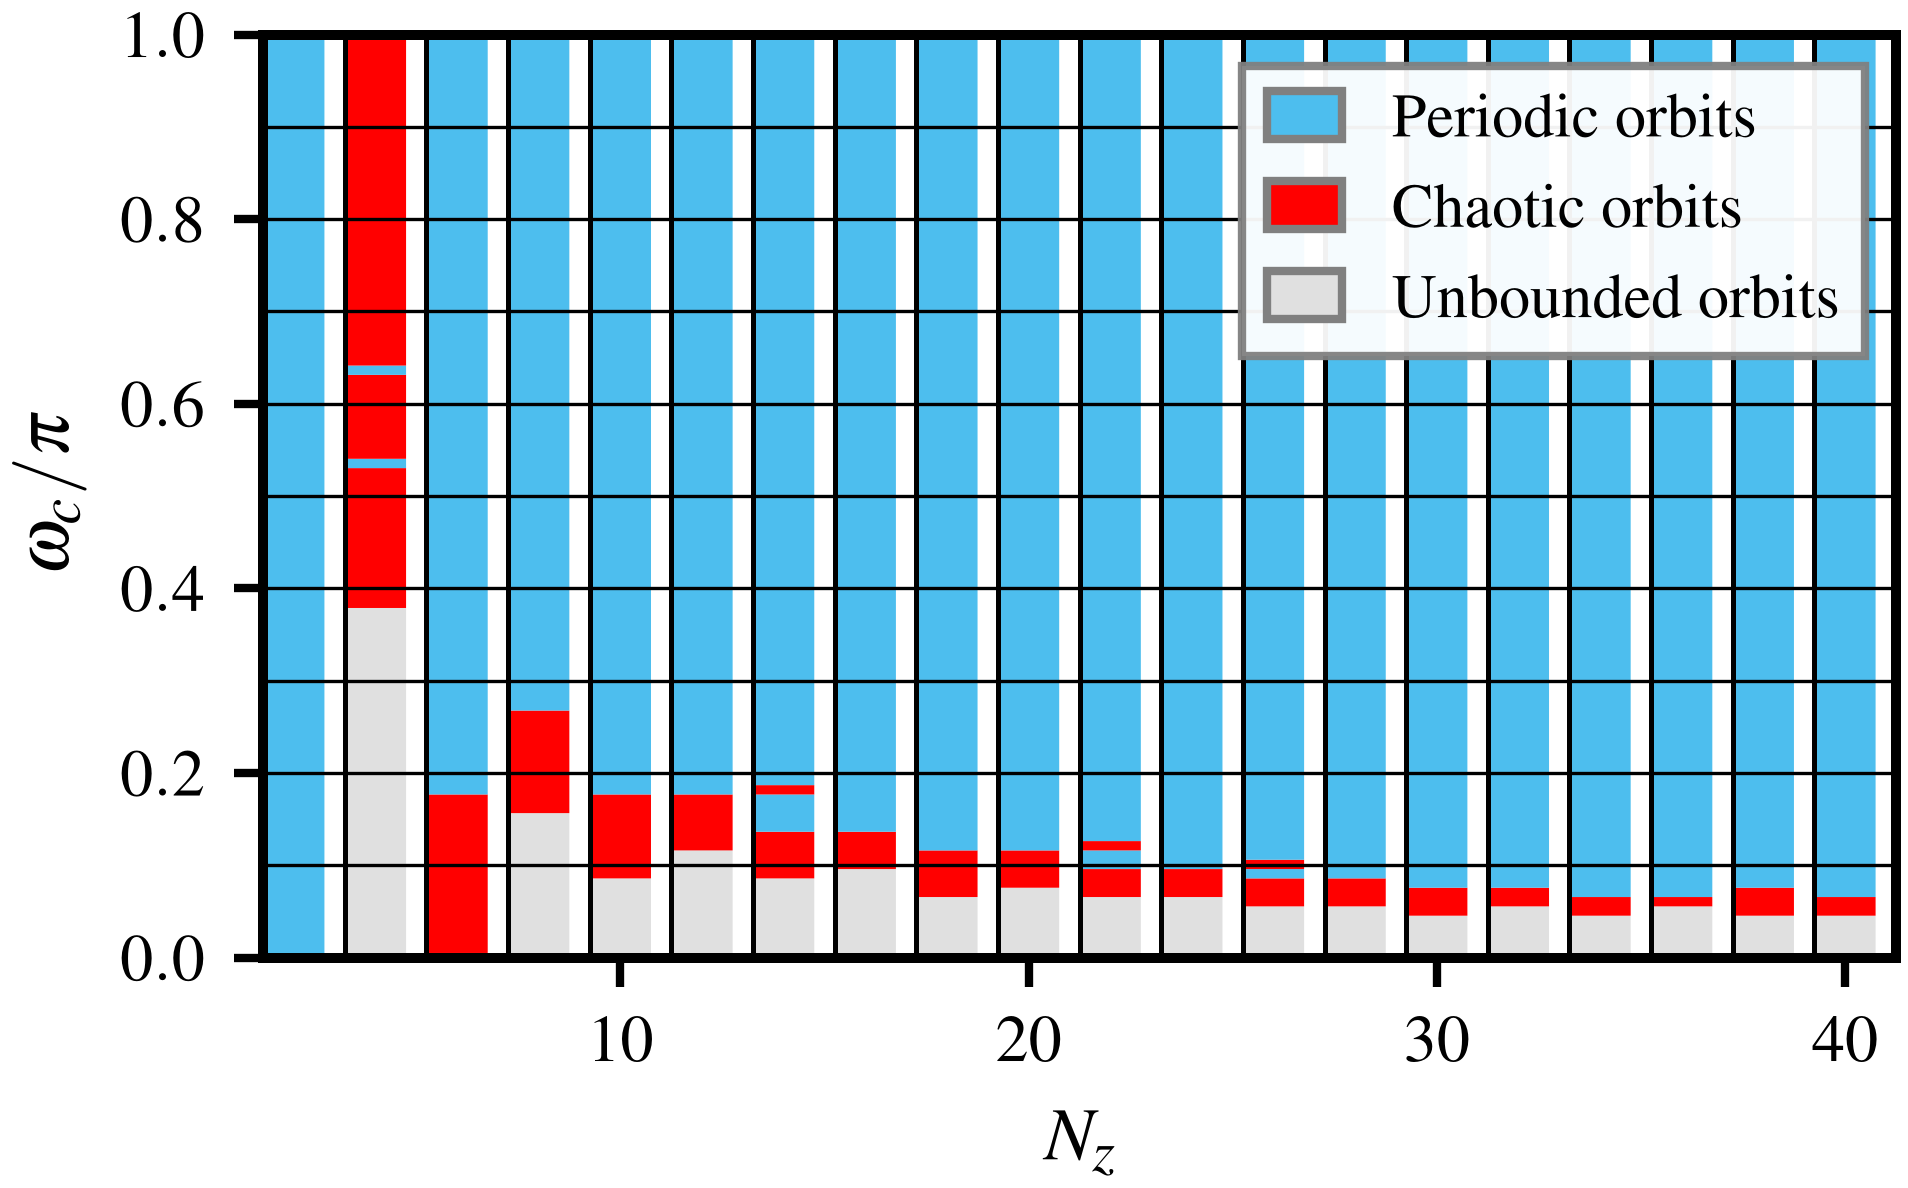
\includegraphics[width=\columnwidth]{Figures/kaiser_b11p5_highpass_classification_interleaved.png}
\caption{Highpass, Kaiser ($\beta_K=11.5$). Reduced chaotic coverage
($\rho_c^{\text{abs}}=7.5\%$), concentrated at $\omega_c/\pi\lesssim 0.5$ and
low orders, with the maximum at the lower edge of the swept interval---behavior opposite to that of the lowpass filter.}
\label{fig:highpass}
\end{figure}

Figure~\ref{fig:bandpass} shows the map for the bandpass filter with the same
Kaiser window ($\beta_K=13.5$), in which a fragmented chaotic structure and
greater sensitivity to variations of $\omega_c$ are observed, consistent with
the narrow band ($\Delta\omega = 0.05\,\pi$) imposed by the filter.

\begin{figure}[!t]
\centering
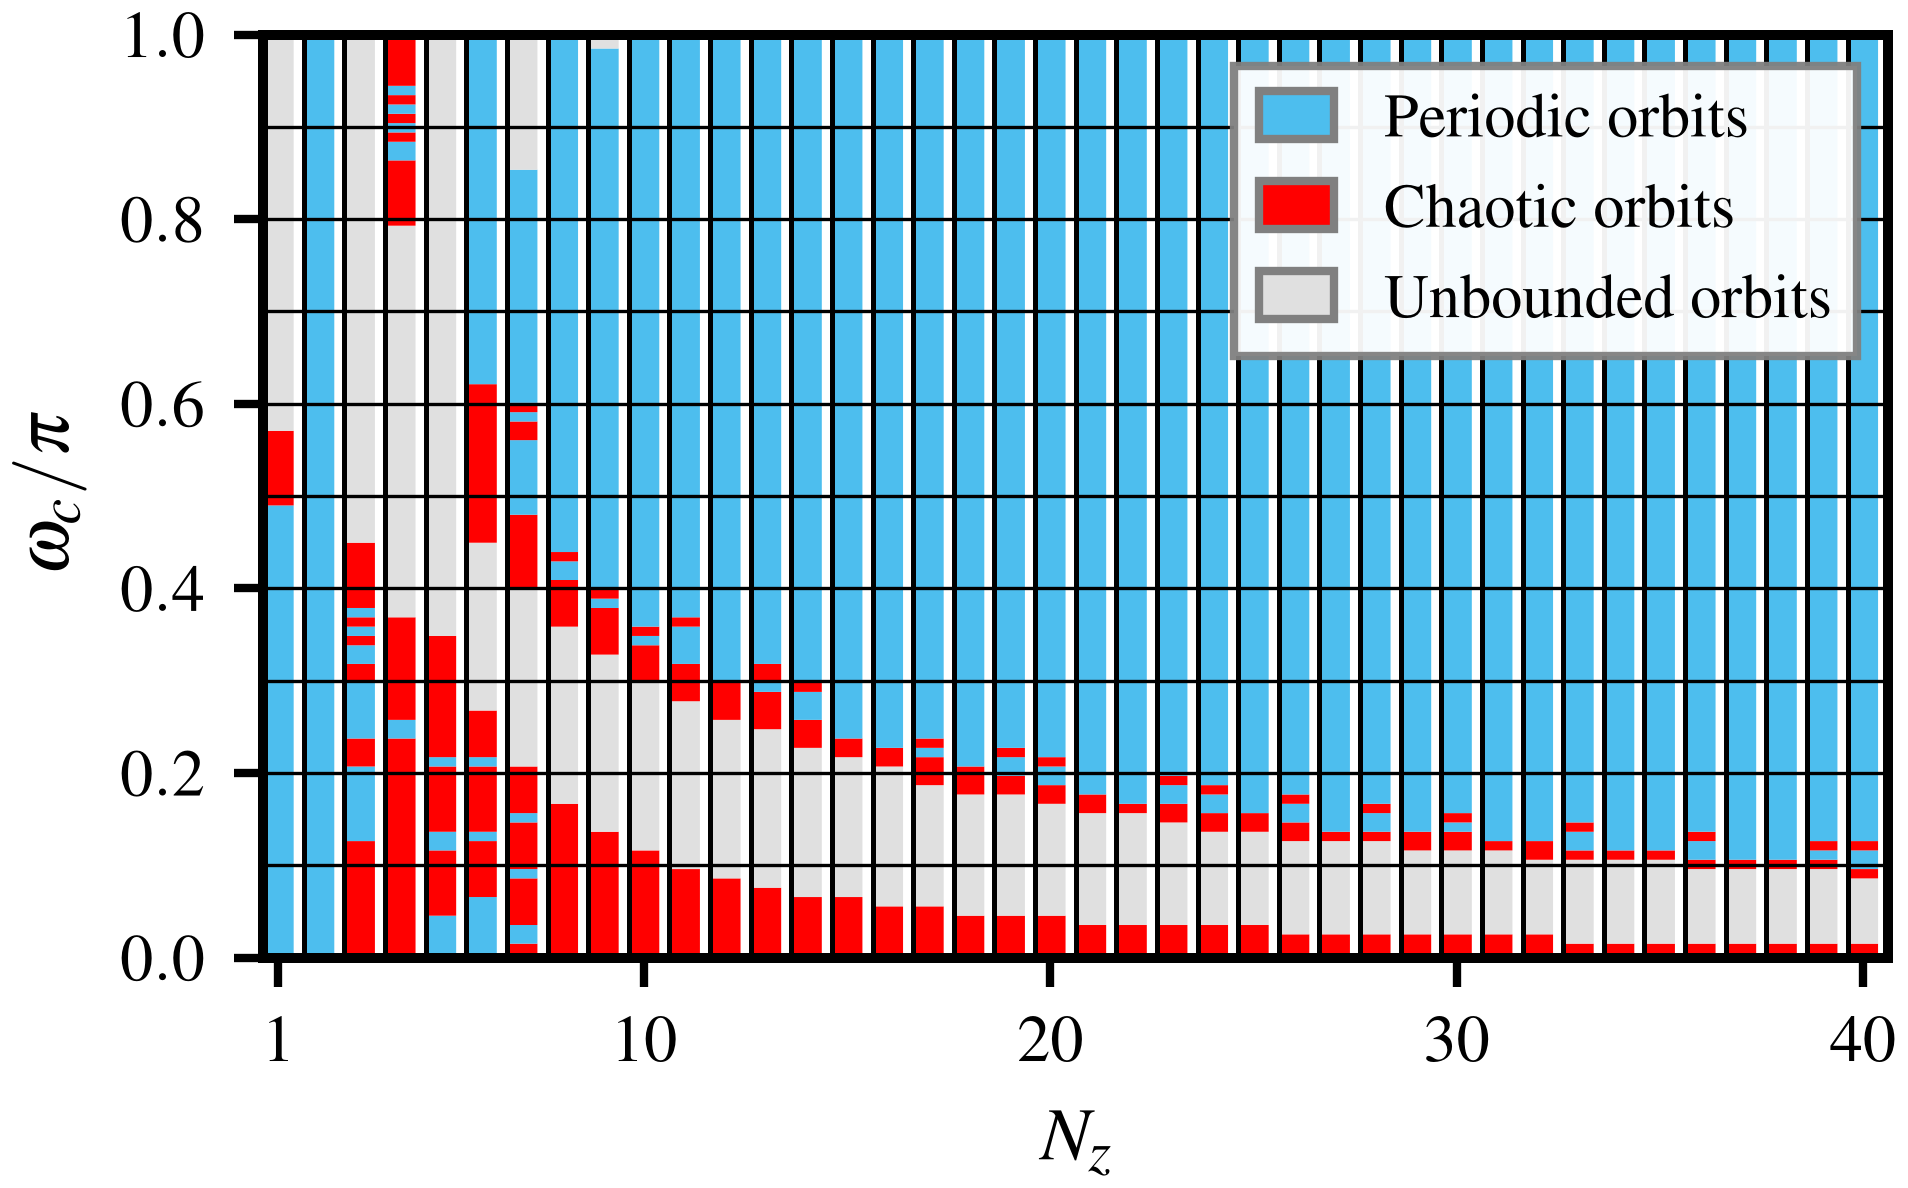
\includegraphics[width=\columnwidth]{Figures/kaiser_b13p5_bandpass_classification_interleaved.png}
\caption{Bandpass, Kaiser ($\beta_K=13.5$), $\Delta\omega=0.05\,\pi$.
Fragmented chaotic structure and greater sensitivity to $\omega_c$; maximum
$\lambda_1$ equal to $0.196$.}
\label{fig:bandpass}
\end{figure}

Figure~\ref{fig:bandstop}, finally, shows the map for the bandstop filter with
the rectangular window. Its conditional coverage $\rho_c^{\text{fin}}=65.2\%$ is
the highest among all evaluated types, even though the absolute coverage is
modest ($5.9\%$) because of the high fraction of divergent points in the grid.

\begin{figure}[!t]
\centering
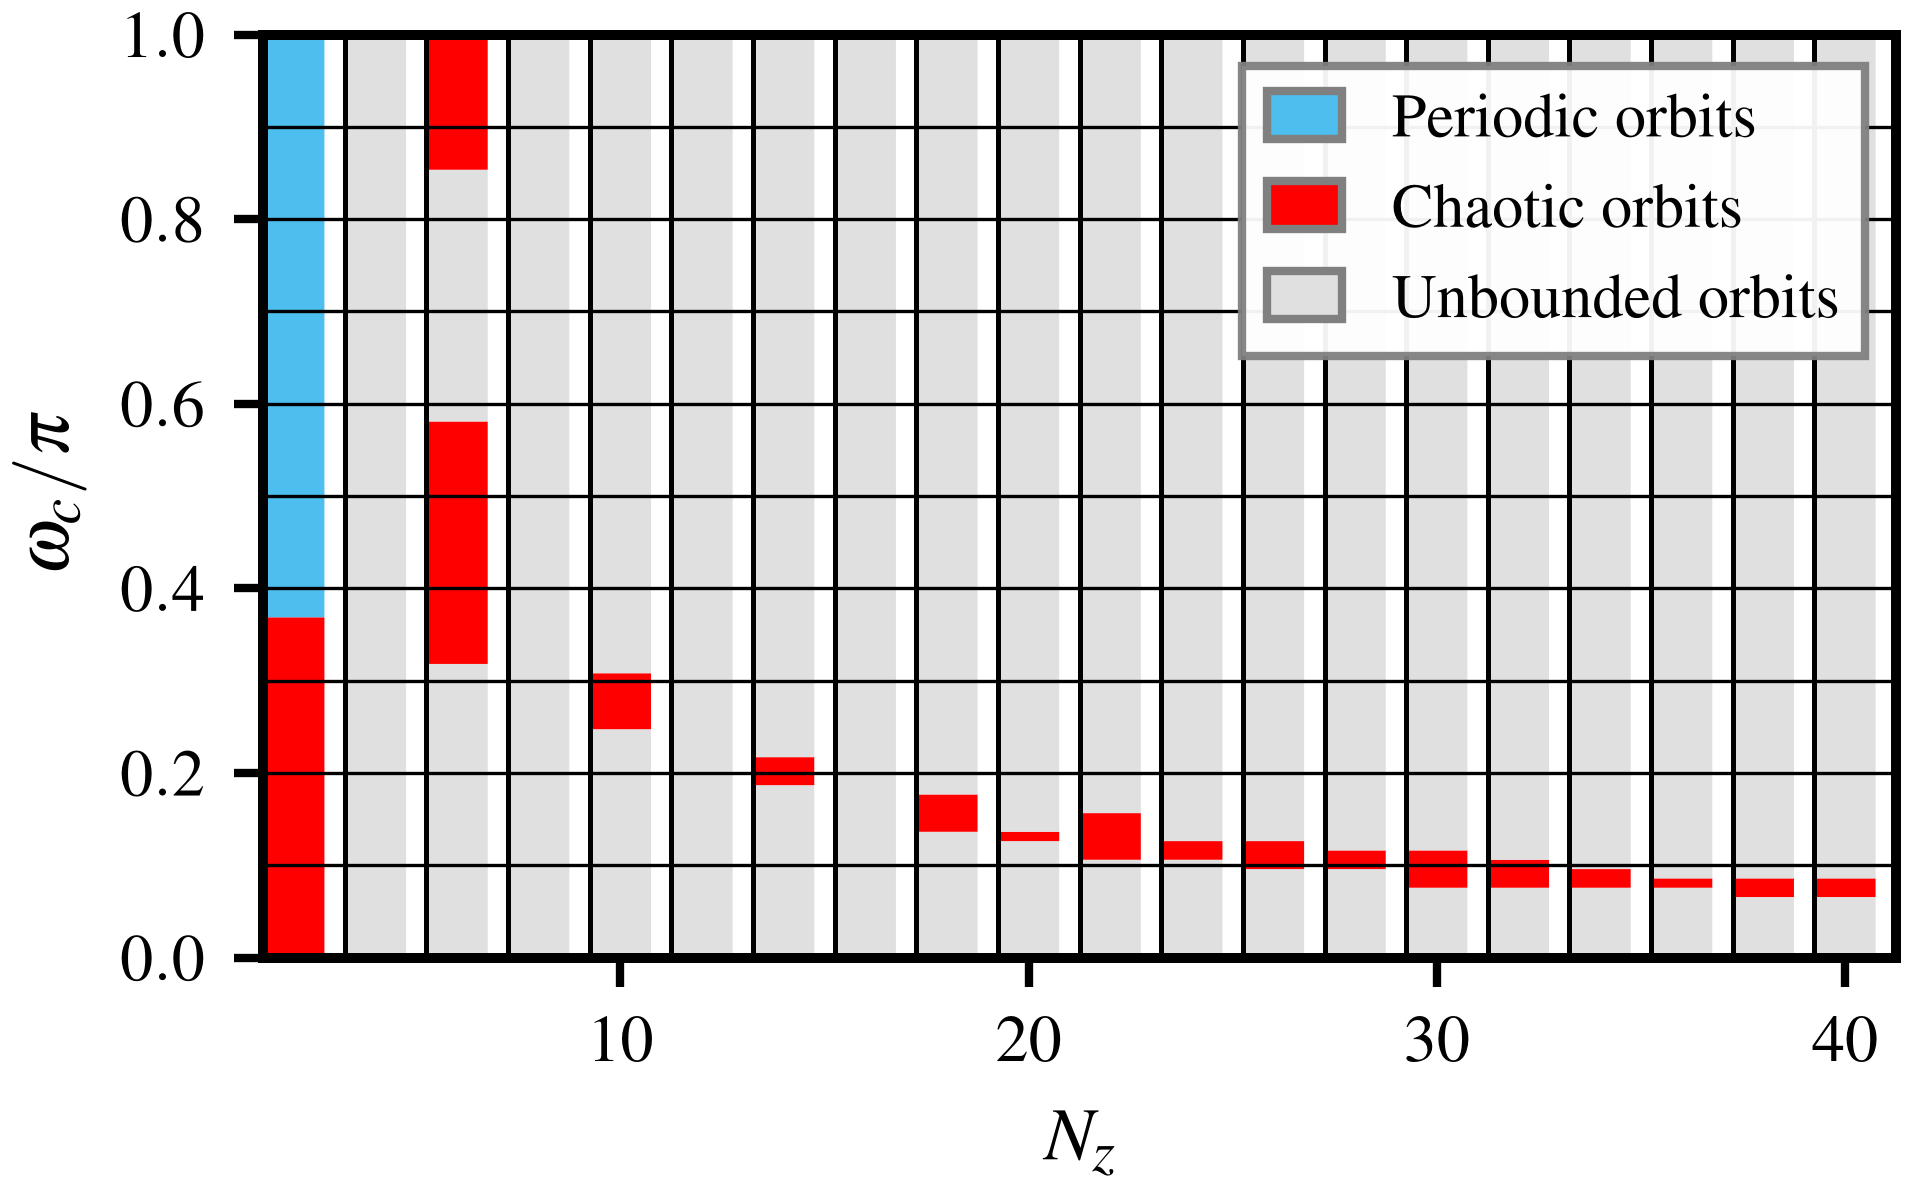
\includegraphics[width=\columnwidth]{Figures/rectangular_bandstop_classification_interleaved.png}
\caption{Bandstop, rectangular window, $\Delta\omega=0.05\,\pi$. Highest
$\rho_c^{\text{fin}}$ among all types ($65.2\%$; $\rho_c^{\text{abs}}=5.9\%$);
absence of a divergent region at low orders.}
\label{fig:bandstop}
\end{figure}

The four filter types differ substantially in the measured composition of the
parameter grid. Pooling the 124 sweeps, the counts per type are: lowpass,
$20{,}906$ chaotic, $17{,}701$ periodic, and $85{,}393$ divergent cells out of
$124{,}000$ ($68.87\%$ divergent); highpass, $2{,}900$, $54{,}902$, and
$4{,}198$ out of $62{,}000$ ($6.77\%$); bandpass, $10{,}219$, $100{,}990$, and
$12{,}791$ out of $124{,}000$ ($10.32\%$); and bandstop, $1{,}598$, $3{,}035$,
and $57{,}367$ out of $62{,}000$ ($92.53\%$). A cell is marked divergent when
at least one of the 25 initial conditions produces a non-finite state during the
$500$ burn-in iterations. In the bandpass case, the chaotic set is limited
predominantly by periodic orbits rather than by divergence ($100{,}990$
periodic against $12{,}791$ divergent cells). The total gain
$G = \sum_j c_j$ equals the filter frequency response at $\omega = 0$, i.e., its
DC gain~\cite{Oppenheim2009}, and the positive equilibrium point
$\mathbf{p}^+$ of the expanded system depends on $G$, as established
analytically by Borges \textit{et al.}~\cite{BorgesCNSNS2024} and recalled in
Subsection~\ref{sub:henon}.

% ---- 4.4 ----
\subsection{Aggregate Analysis and Chaotic Density}\label{sub:density}
From the individual maps, all points classified as chaotic in each of the 124
sweeps (4 filter types $\times$ 6 fixed windows $+$ 4 types $\times$ 25 values
of $\beta_K$ of the Kaiser window) were aggregated in the $(N_z,\omega_c/\pi)$
plane, regardless of the window or filter type. The result is the chaotic
density map of Figure~\ref{fig:density}, which indicates which regions of the
parameter space are classified as chaotic in the largest number of
configurations.

\begin{figure}[!t]
\centering
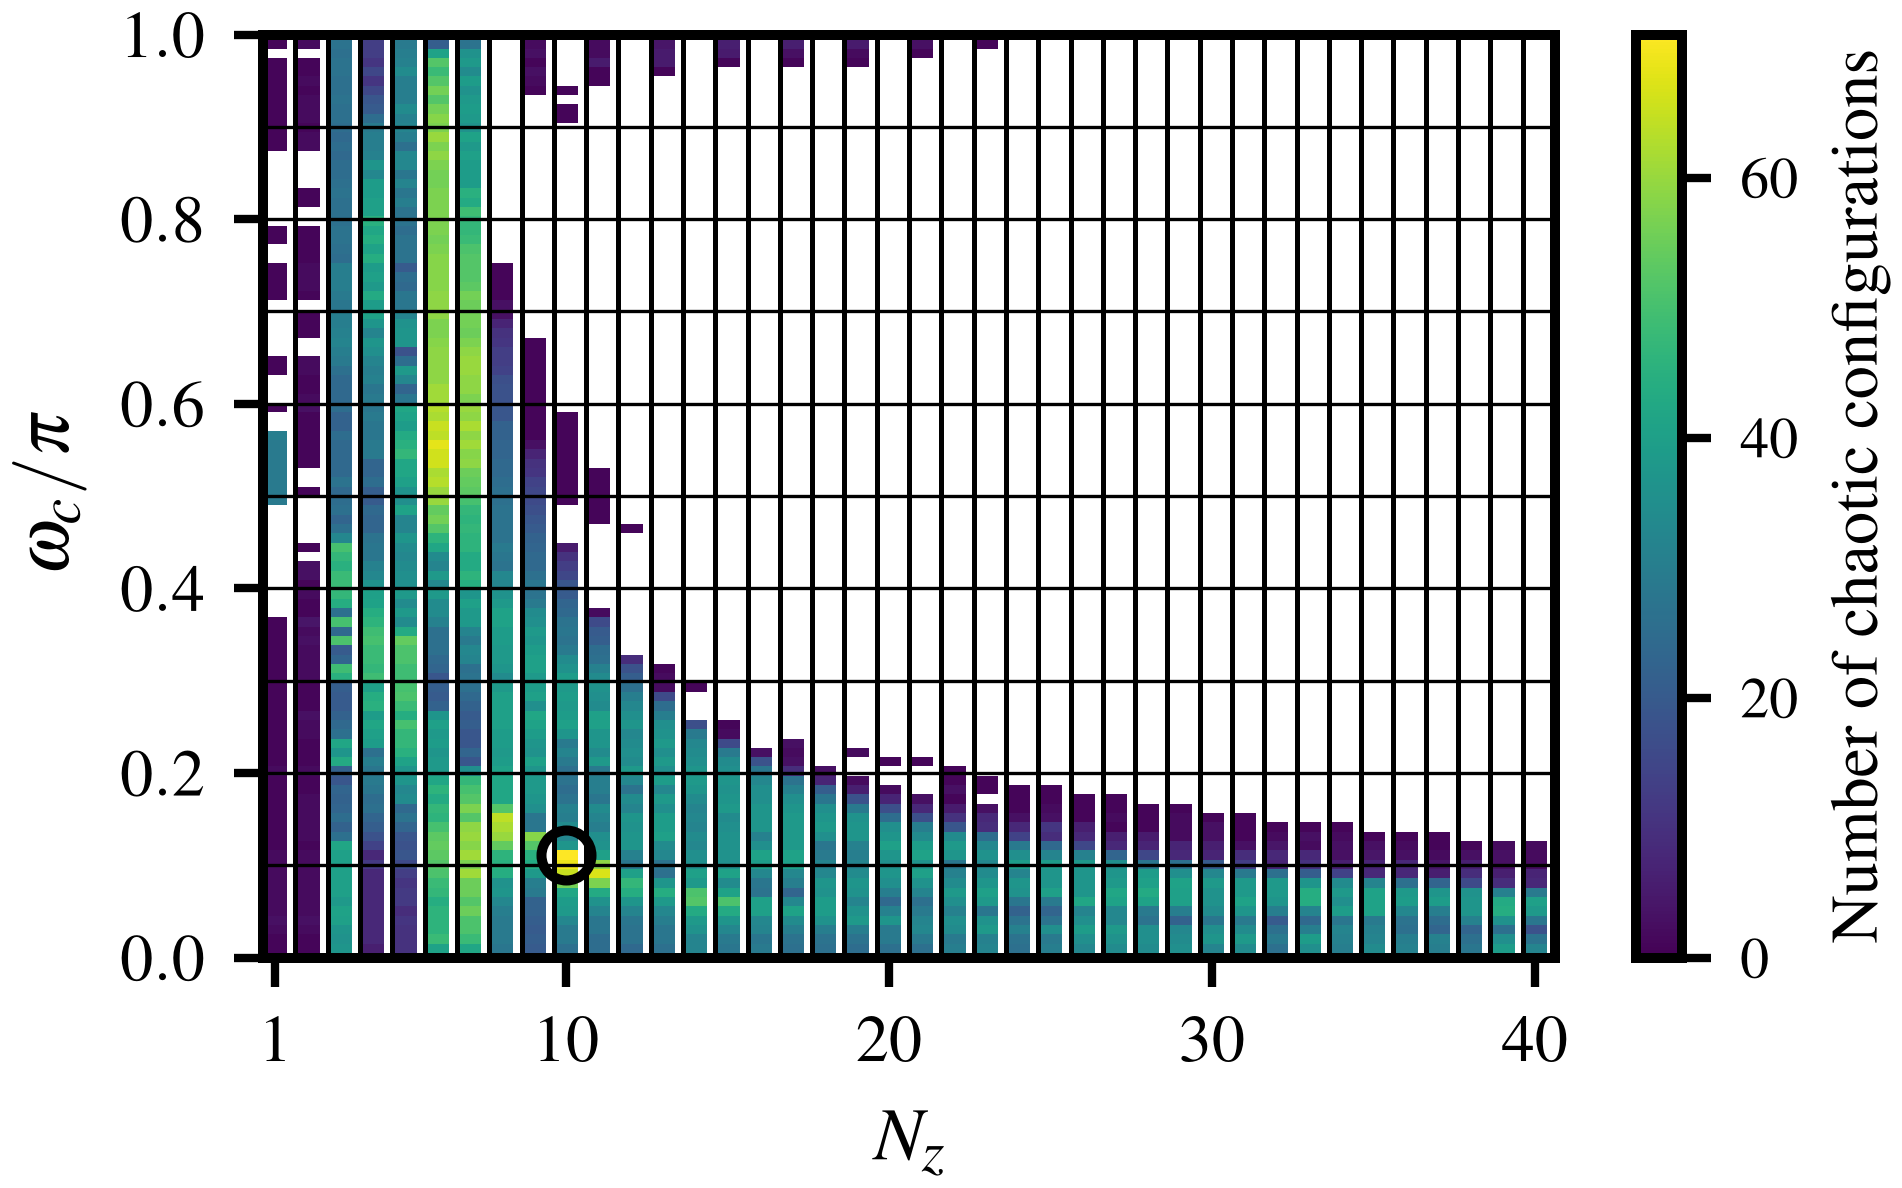
\includegraphics[width=\columnwidth]{Figures/fig_chaotic_density.png}
\caption{Aggregate chaotic density over the 124 sweeps. Light tones indicate
regions that are chaotic in a larger number of configurations; dark tones
indicate fewer. The marker ($\circ$) highlights the point of maximum density,
classified as chaotic in 71 of the 124 configurations.}
\label{fig:density}
\end{figure}

The density map shows that the regions in which the chaotic regime is sustained
across most of the windows and filter types are concentrated at intermediate-to-high
cutoff frequencies and at moderate orders, regardless of the window or filter
type. For high $N_z$, all configurations converge to similar dynamic
behavior---a reflection of the approach to the ideal
filter~\cite{Oppenheim2009}---indicating that the choice of the window is a
relevant design parameter mainly in the low-to-moderate order ranges.

The presence of \textit{shrimps}~\cite{Gallas1993,BorgesCSF2022} and of
bifurcation boundaries that are finely interleaved---formed by period-doubling
cascades alternating with shrimp-shaped periodic islands at progressively
smaller scales~\cite{Gallas1993,BorgesCSF2022}---implies that small variations
of $N_z$ or $\omega_c$ can move a configuration across a regime boundary, so the
distance from each operating point to the nearest such boundary becomes an
auxiliary design parameter.

% ---- 4.5 ----
\subsection{Effect of the Kaiser-Window Parameter $\beta_K$}\label{sub:beta}
The Kaiser window is the only one of the seven evaluated that has a continuous
shape parameter, $\beta_K$, providing a one-dimensional path through the space
of windows~\cite{Kaiser1980}: for $\beta_K=0$ it coincides with the rectangular
window and, as $\beta_K$ grows, the stopband attenuation increases at the
expense of widening the main lobe~\cite{Oppenheim2009}. This subsection examines
how the chaotic coverage responds to this parameter, based on the dedicated
sweep described in Subsection~\ref{sub:types}, in which $\beta_K$ covers the
interval $[2.0,14.0]$ over 25 values for the four filter types.

The values of $\beta_K$ that maximize the number of chaotic points $N_c$ per
filter type, reported in Table~\ref{tab:best}, are $\beta_K=13.5$ for lowpass
and bandpass, $\beta_K=11.5$ for highpass, and $\beta_K=4.0$ for bandstop. For
the first three types, the maximum lies at high values of $\beta_K$, where the
window presents side lobes with strong attenuation~\cite{Oppenheim2009}---behavior
consistent with the finding of Subsection~\ref{sub:classification} that windows of
higher spectral attenuation, such as Blackman--Harris, favor the preservation of
the chaotic regime in these three filter types. For lowpass in particular, it was
observed that the absolute coverage $\rho_c^{\text{abs}}$ grows sharply with
$\beta_K$ until it stabilizes at an approximate plateau for $\beta_K$ between about
$11$ and $14$, a range that contains the value $\beta_K=13.5$ of largest $N_c$.

The distinct behavior of the bandstop filter, whose maximum $N_c$ occurs with the
rectangular window and, among the Kaiser configurations, at $\beta_K=4.0$
(Table~\ref{tab:best}), suggests a different interpretation: for filtering
geometries that remove only a narrow band of the spectrum, the preservation of
most of the spectral energy in the feedback loop seems to weigh more than the
depth of the stopband attenuation---a hypothesis coherent with the best
performance of the rectangular window, of lowest attenuation, in this same
filter type. This difference reinforces that the effect of $\beta_K$ is not
monotonic across the four filter types, depending on the geometry of the imposed
spectral mask.

% ---- 4.6 ----
\subsection{Statistical Confidence and Configuration Ranking}\label{sub:ranking}
The previous subsections reported, for each filter type, the configuration of
greatest chaotic coverage. This subsection quantifies the statistical confidence
of those estimates and consolidates the ordering of all window--filter
combinations into a single reference table.

For each combination, the regional mean of $\lambda_1$ over the chaotic grid
points (sample size $N_c$) is accompanied by a 95\% confidence interval obtained
by nonparametric bootstrap~\cite{EfronTibshirani1993} with $1{,}000$ resamples
(seed $42$), as defined in Subsection~\ref{sub:stats}. In all reported chaotic
configurations, the confidence interval of $\bar\lambda_1$ lies entirely above
zero---for example, $[0.0223,\,0.0254]$ for lowpass with Kaiser ($\beta_K=13.5$)
and $[0.0627,\,0.0800]$ for bandstop with the rectangular window
(Table~\ref{tab:best})---confirming that the regional mean is positive with
statistical confidence. The standard deviation $\sigma_{\lambda_1}$, being the
spatial dispersion of $\lambda_1$ over the chaotic region, informs its
homogeneity: the rectangular bandstop presents the highest value
($\sigma_{\lambda_1}=0.0491$), reflecting the coexistence of low and high
$\lambda_1$ in its fragmented chaotic region, while the lowpass with Kaiser
exhibits a smaller dispersion ($\sigma_{\lambda_1}=0.0231$) over a more
homogeneous region.

The per-type trends are read directly from the classification maps and the
per-type sweet spots: in lowpass filters the chaotic region concentrates at
higher cutoff frequencies, whereas in highpass filters it migrates to low
cutoff frequencies, with the highpass sweet spot located at
$\omega_c/\pi\approx 0.01$ (Figs.~\ref{fig:lowpass} and~\ref{fig:highpass}).
The per-configuration statistics are reproduced by the released
package~\cite{chaoticPFC2026}.

Table~\ref{tab:ranking} consolidates the ranking of the window--filter
configurations, considering the six fixed-coefficient windows and the best Kaiser
window of each filter type, ordered by the number of chaotic points $N_c$.

\begin{table*}[!t]
\caption{Ranking of the Window--Filter Combinations (Fixed Windows and Best Kaiser per Filter Type), by $N_c$\label{tab:ranking}}
\centering
\begin{tabular}{rllrrrc}
\toprule
\textbf{\#} & \textbf{Filter} & \textbf{Window} & $N_c$ &
$\rho_c^{\text{fin}}$ & $\bar\lambda_1$ & 95\% CI \\
\midrule
 1 & Lowpass   & Kaiser ($\beta_K{=}13.5$) & 979 & 77.6\% & 0.0239 & $[0.0223,\,0.0254]$ \\
 2 & Lowpass   & Blackman--Harris          & 961 & 74.8\% & 0.0211 & $[0.0197,\,0.0227]$ \\
 3 & Lowpass   & Blackman                  & 801 & 61.8\% & 0.0176 & $[0.0160,\,0.0193]$ \\
 4 & Lowpass   & Hann                      & 606 & 51.2\% & 0.0190 & $[0.0170,\,0.0208]$ \\
 5 & Lowpass   & Bartlett                  & 458 & 41.3\% & 0.0198 & $[0.0174,\,0.0226]$ \\
 6 & Lowpass   & Hamming                   & 450 & 35.9\% & 0.0263 & $[0.0240,\,0.0290]$ \\
 7 & Bandpass  & Kaiser ($\beta_K{=}13.5$) & 434 & 13.0\% & 0.0286 & $[0.0258,\,0.0315]$ \\
 8 & Bandpass  & Blackman--Harris          & 418 & 12.3\% & 0.0261 & $[0.0235,\,0.0293]$ \\
 9 & Bandpass  & Blackman                  & 394 & 11.1\% & 0.0252 & $[0.0218,\,0.0290]$ \\
10 & Bandpass  & Hamming                   & 294 &  7.9\% & 0.0273 & $[0.0235,\,0.0315]$ \\
11 & Bandpass  & Hann                      & 288 &  8.0\% & 0.0267 & $[0.0231,\,0.0311]$ \\
12 & Bandpass  & Bartlett                  & 249 &  6.9\% & 0.0293 & $[0.0254,\,0.0337]$ \\
13 & Lowpass   & Rectangular               & 204 & 19.5\% & 0.0354 & $[0.0314,\,0.0396]$ \\
14 & Highpass  & Kaiser ($\beta_K{=}11.5$) & 149 &  8.1\% & 0.0178 & $[0.0138,\,0.0219]$ \\
15 & Highpass  & Blackman--Harris          & 144 &  7.9\% & 0.0190 & $[0.0151,\,0.0237]$ \\
16 & Bandpass  & Rectangular               & 141 &  3.7\% & 0.0153 & $[0.0113,\,0.0211]$ \\
17 & Bandstop  & Rectangular               & 118 & 65.2\% & 0.0709 & $[0.0627,\,0.0800]$ \\
18 & Highpass  & Blackman                  &  97 &  5.2\% & 0.0216 & $[0.0170,\,0.0277]$ \\
19 & Highpass  & Bartlett                  &  86 &  4.6\% & 0.0237 & $[0.0186,\,0.0299]$ \\
20 & Highpass  & Hann                      &  79 &  4.2\% & 0.0233 & $[0.0173,\,0.0310]$ \\
21 & Highpass  & Hamming                   &  72 &  3.8\% & 0.0234 & $[0.0175,\,0.0300]$ \\
22 & Bandstop  & Kaiser ($\beta_K{=}4.0$)  &  58 & 39.2\% & 0.0726 & $[0.0626,\,0.0798]$ \\
23 & Bandstop  & Hamming                   &  55 & 35.5\% & 0.0874 & $[0.0854,\,0.0892]$ \\
24 & Bandstop  & Blackman                  &  50 & 33.3\% & 0.0888 & $[0.0865,\,0.0912]$ \\
25 & Bandstop  & Hann                      &  49 & 32.9\% & 0.0877 & $[0.0860,\,0.0896]$ \\
26 & Bandstop  & Blackman--Harris          &  47 & 32.0\% & 0.0929 & $[0.0909,\,0.0946]$ \\
27 & Bandstop  & Bartlett                  &  43 & 30.1\% & 0.0896 & $[0.0882,\,0.0911]$ \\
28 & Highpass  & Rectangular               &  25 &  1.3\% & 0.0269 & $[0.0171,\,0.0398]$ \\
\bottomrule
\end{tabular}

\vspace{2pt}
{\footnotesize 95\% intervals by
bootstrap~\cite{EfronTibshirani1993}. Full per-configuration tables are regenerated from the versioned
checkpoints by the released package~\cite{chaoticPFC2026}.}
\end{table*}

The ranking in Table~\ref{tab:ranking} shows that the first six positions are
all of the lowpass type, confirming it as the filter of greatest absolute
chaotic coverage, and that highpass and bandstop occupy mostly the lower half of
the table. A relevant contrast for CBCS design is also observed: although the
bandstop filter occupies low positions in $N_c$, its configurations present the
highest values of $\bar\lambda_1$ (up to $0.0929$), indicating that, when
chaotic, their orbits exhibit greater sensitivity to initial conditions than
those of the lowpass filter---a potentially desirable property depending on the
application.

% ---- 4.7 ----
\subsection{Computational Cost and Reproducibility}\label{sub:cost}
The complete sweep, comprising 124 window--filter combinations with an average
grid of 3{,}000 points $\times$ 25 initial conditions $\times$ up to 3{,}000
iterations of the Lyapunov estimator, totaled approximately $2.8\times 10^{10}$
iterations of the expanded map and $3.5\times 10^{11}$ Jacobian--basis
operations. With cores compiled via Numba~\cite{Numba} and parallelization over
the threads available on the reference machine (an 8th-generation Intel Core i7
processor with 6 physical cores and 12 logical threads, 16\,GB of RAM), the total
execution time was on the order of 6\,h. Relative to an equivalent pure-Python
implementation (without JIT), the package microbenchmarks during development
indicated a reduction of one to two orders of magnitude in execution time---the
reason for the architectural decision discussed in Subsection~\ref{sub:arch}.

All the infrastructure is versioned in the repository: sweep checkpoints in
\texttt{data/sweeps/}, figure-generation scripts in
\texttt{src/chaotic\_pfc/sweep\_plotting.py}, tests in \texttt{tests/}, and
documentation in \texttt{docs/} (published on Read the Docs). The
reproducibility of any figure or table of the present work can be obtained by
running the corresponding script over the versioned checkpoint, without the
need to recompute the sweep.

Taken together, the results of the previous subsections consolidate a
characterization of the parameter space of the FIR-filtered H\'enon map that is
broader than the one documented in the previous literature; their implications
are summarized in the following section.

% ============================================================
\section{Final Remarks}\label{sec:conclusion}
% ============================================================
The dynamics of the H\'enon map with FIR filters inserted in the feedback loop
were investigated numerically, extending the results of Borges \textit{et
al.}~\cite{Borges2022sbrt} and~\cite{BorgesCNSNS2024}, which vary the
zero-placement geometry of the FIR filter with a fixed design window, to a
higher-dimensional design space:
four filter types (lowpass, highpass, bandpass, and bandstop) and seven windows
(rectangular, Bartlett, Hamming, Hann, Blackman, Blackman--Harris, and Kaiser
with a dedicated sweep of the shape parameter $\beta_K$).

It was confirmed that the insertion of the filters can substantially alter the
nature of the generated signals, producing convergence to stationary regimes,
periodic orbits, or chaotic behavior, depending on the adopted
$(N_z,\omega_c/\pi)$ combination. The chaotic regime is not eliminated by the
filtering, but rather reorganized into well-defined regions of the parameter
space, dependent on the filter type and the window. For lowpass and bandpass
filters, the Kaiser window with high $\beta_K$ maximizes the chaotic coverage,
reaching $\rho_c^{\text{abs}} = 24.5\%$ in the lowpass case---the highest
absolute coverage among all configurations. For the bandstop filter, the
rectangular window surpasses the others in conditional terms
($\rho_c^{\text{fin}} = 65.2\%$), although its absolute coverage is modest
($5.9\%$).

The aggregate analysis over the 124 sweeps revealed that the regions in which
the chaotic regime is sustained across most of the windows and filter types are
concentrated at intermediate-to-high cutoff frequencies and moderate orders. The
bootstrap confidence intervals on $\lambda_1$ place the regional mean of every
reported chaotic configuration strictly above zero; read per filter
type from the classification maps, the chaotic region migrates toward higher
cutoff frequencies for the lowpass filter and toward lower ones for the highpass
filter. The presence of
\textit{shrimps}~\cite{Gallas1993} and of finely interleaved bifurcation
boundaries reinforces the need for explicit verification of the generator
dynamics after the insertion of linear filters---the preservation of chaos
cannot be presumed.

\textit{Synthesis thesis.} The joint choice of the filter type and the design
window is a first-order parameter for the dynamic behavior of filtered H\'enon
generators: given the finely interleaved transition boundaries and the
existence of \textit{shrimps} inside the chaotic regions, the design of CBCS with
filtering cannot start solely from the spectral specification of the filter; it
requires explicit verification of the dynamics of the resulting generator by
means of the classification maps produced here. The divergent fraction of the
grid measured over the 124 sweeps ranges from $6.77\%$ (highpass) and $10.32\%$
(bandpass) to $68.87\%$ (lowpass) and $92.53\%$ (bandstop), with the counts
reported in Subsection~\ref{sub:maps}.

\textit{Acknowledged limitations.} The sweeps cover $N_z\le 40$ and horizons of
$N_{\text{map}}\le 3{,}000$ iterations; much higher orders and unbounded horizons
could reveal additional structures. The band width $\Delta\omega$ was fixed at
$0.05\,\pi$ for bandpass and bandstop; variations of this parameter may produce
qualitative transitions in the conclusions for these two filter types. The choice
of the canonical parameters $(\alpha,\beta) = (1.4,0.3)$ of the underlying map was
not swept; other pairs in the parameter space of the H\'enon
map~\cite{Gallas1993} may present qualitatively distinct behaviors under
filtering. The regional mean $\bar\lambda_1$ is computed only over the initial
conditions that survive the accumulation window: initial conditions that diverge
after the burn-in are discarded from the average, so $\lambda_1$ is estimated
over the survivors. The sampling neighborhood of the initial conditions is a cube
of edge $0.1$, in contrast to the sphere of radius $0.01$ used by Borges
\textit{et al.}~\cite{BorgesCNSNS2024}.

\textit{Future work.} Three directions are highlighted: (a)~sweeping the band
width $\Delta\omega$ as an independent variable for bandpass and bandstop filters,
with the possibility of identifying additional transitions and dynamic resonances
not captured in this study; (b)~extending the parametric-sweep methodology to
infinite-impulse-response (IIR) filters, whose dynamic behavior is still little
explored in the literature~\cite{Borges2024sbrt}, with explicit treatment of
filter stability beyond map stability; and (c)~a systematic spectral
characterization of all the chaotic configurations identified, measuring occupied
bandwidth, spectral leakage, and in-band power ratios as auxiliary metrics to
$\lambda_1$ for the selection of operating points in CBCS.

% ============================================================
% REFERENCES
% ============================================================
% JCIS requires a DOI for every reference. Keep referencias.bib up to date
% and add the DOI field to each entry; IEEEtran.bst will render it.
\bibliographystyle{IEEEtran}
\bibliography{references}

\end{document}